%
%Final - 2 column style
\documentclass[utf8]{frontiersSCNS} % for Science, Engineering and Humanities and Social Sciences articles

% For using overleaf or local compilation
% See setting of true/false directly after \begin{document}
\newif\ifoverleaf % default is \overleaftrue

% The preceding line is only needed to identify funding in the first footnote. If that is unneeded, please comment it out.
\usepackage{acronym}
\usepackage{algorithm}
\usepackage{algpseudocode}
\usepackage{amsmath}
\usepackage{amsmath, amssymb,longtable,dcolumn, nccmath}
\usepackage{balance}
\usepackage{bm}
%\usepackage[caption=false,font=footnotesize]{subfig}
\usepackage{cite}
\usepackage{colortbl}
\usepackage{csvsimple}
%\usepackage{enumitem} % also breaks things
\usepackage{fancyhdr}
%\usepackage{fixltx2e}
\usepackage{fullpage}
\usepackage{graphicx} 
%\usepackage{hyperref}  % Seems to break things
\usepackage{indentfirst}
\usepackage{multirow}
\usepackage{natbib}
\usepackage{pdfpages}
%\usepackage{stfloats}  % Written by Sigitas Tolusis
%\usepackage{subcaption}
%\usepackage{subfigure}
\usepackage{tabularx}
\usepackage{times}
\usepackage{units}
\usepackage{siunitx}

% Requires sudo apt-get install texlive-publishers texlive-publishers-doc
\usepackage{IEEEtrantools}

% For Frontiers
\usepackage{url,hyperref,lineno,microtype,subcaption}
\usepackage[onehalfspacing]{setspace}
\usepackage{xcolor}
%\linenumbers

% Load this package last - for non-line-break hyphens (e.g., WAM-V)
% See https://tex.stackexchange.com/questions/103608/how-to-force-latex-not-to-break-the-line-after-a-hyphen
\usepackage[shortcuts]{extdash}

\def\keyFont{\fontsize{8}{11}\helveticabold }
\def\firstAuthorLast{Sample {et~al.}} %use et al only if is more than 1 author
\def\Authors{Brian Bingham\,$^{1,*}$, Carlos Ag{\"u}ero\,$^{2}$, Michael McCarrin\,$^{1}$, Joseph Klamo\,$^{1}$, Joshua Malia\,$^{1}$, Woensug Choi\,^{1}, Kevin Allen\,$^{3}$, Tyler Lum\,$^{4}$, Marshall Rawson\,$^{3}$ and Rumman Waqar\,$^{5}$}
% Affiliations should be keyed to the author's name with superscript numbers and be listed as follows: Laboratory, Institute, Department, Organization, City, State abbreviation (USA, Canada, Australia), and Country (without detailed address information such as city zip codes or street names).
% If one of the authors has a change of address, list the new address below the correspondence details using a superscript symbol and use the same symbol to indicate the author in the author list.
\def\Address{$^{1}$Naval Postgraduate School, $^{2}$Open Robotics, $^{3}$University of Florida, $^{4}$University of British Columbia, $^{5}$University of London}
% The Corresponding Author should be marked with an asterisk
% Provide the exact contact address (this time including street name and city zip code) and email of the corresponding author
\def\corrAuthor{Brian Bingham}
\def\corrEmail{bbingham@nps.edu}
%
\begin{document}

%\overleaffalse
\overleaftrue

% A few math shortcuts
% Stolen from Austratlian Center for Field Robotics
% Thanks Alex!
% bbing 24.02.03

% general global definitions
\newcommand{\Def}{\ {\buildrel \triangle\over =}\ }
\newcommand{\beq} {\begin{equation}}
\newcommand{\eeq} {\end{equation}}
%\newcommand{\beqn} {\begin{eqnarray}}
%\newcommand{\eeqn} {\end{eqnarray}}
%\newcommand{\E}[1] {\mbox{$ {\rm E} \{ #1 \}$ }}
\newcommand{\Es}[2] {\mbox{$ {\rm E}^{#1} \{ #2 \}$ }}
\newcommand{\Set}[1] {\mbox{$ \{ #1 \} $ }}
\newcommand{\Cal}[1] {\mbox{$ {\cal #1 } $}}
\newcommand{\PR}[1]  {\mbox{$ P(#1) $}}
\newcommand{\Pri}[2]  {\mbox{$ P_{#1}(#2) $}}
\newcommand{\PRi}[2]  {\mbox{$ P_{#1}(#2) $}}
\newcommand{\Pris}[3]  {\mbox{$ P_{#1}^{#2}(#3) $}}
\newcommand{\like}[1]  {\mbox{$ \Lambda(\bf #1) $}}
\newcommand{\likei}[2]  {\mbox{$ \Lambda_{#2}(\bf #1) $}}
\newcommand{\LL}[1]  {\mbox{$ l(#1) $}} % loglikelihood
\newcommand{\LLi}[2]  {\mbox{$ l_{#1}(#2) $}} %loglikelihood
\newcommand{\EN}[1]  {\mbox{$ H(#1) $}} % entropy
\newcommand{\ENi}[2]  {\mbox{$ H_{#1}(#2) $}} % entropy
\newcommand{\mEN}[1]  {\mbox{$ \overline{H}(#1) $}} % mean entropy
\newcommand{\MI}[1]  {\mbox{$ I(#1) $}}  %mutual information
\newcommand{\est}[1]  {\mbox{$\hat{\bf #1}$}}
\newcommand{\estk}[2]  {\mbox{$\hat{\bf #1}(#2)$}}
\newcommand{\D}[1]    {\mbox{${\rm d} {#1}$}}
\newcommand{\mean}[1] {\mbox{$\overline{ #1}$}}
\newcommand{\Det}[1] {\mbox{$\mid {#1} \mid $}}
\newcommand{\One}      {\mbox{${\bf 1}$}}
\newcommand{\Zero}      {\mbox{${\bf 0}$}}
\newcommand{\grad}[1] {\mbox{${\bf\nabla} #1$}}
%\newcommand{\J}[3] {\mbox{${\bf\nabla}{\bf #1}_{\bf #2}(#3)$}}
\newcommand{\Jt}[3] {\mbox{${\bf\nabla}^T{\bf #1}_{\bf #2}(#3)$}}
\newcommand{\pdf}{{\it pdf\ }}
\newcommand{\dxt}[2]  {\mbox{$\dot{\bf #1}( #2)$}}
% defining different types of vectors
% first those with no time subscripts
\renewcommand{\V}[1] {\mbox{${\bf #1}$}}
\newcommand{\Vt}[1] {\mbox{${\bf #1}^T$}}
\newcommand{\Vin}[1] {\mbox{${\bf #1}^{-1}$}}
\newcommand{\Vgin}[1] {\mbox{${\bf #1}^{\dagger}$}}
\newcommand{\Vi}[2] {\mbox{${\bf #1}_{#2}$}}
\newcommand{\Vs}[2] {\mbox{${\bf #1}^{#2}$}}
\newcommand{\Vis}[3] {\mbox{${\bf #1}_{#2}^{#3}$}}
\newcommand{\Vit}[2] {\mbox{${\bf #1}_{#2}^T$}}
\newcommand{\Vini}[2] {\mbox{${\bf #1}_{#2}^{-1}$}}
\newcommand{\Vgini}[2] {\mbox{${\bf #1}^{\dagger}$}}

% next those with time subscript k (very common)
\newcommand{\Vk}[1] {\mbox{${\bf #1}(k)$}}
\newcommand{\Vkt}[1] {\mbox{${\bf #1}^T(k)$}}
\newcommand{\Vkin}[1] {\mbox{${\bf #1}^{-1}(k)$}}
\newcommand{\Vkgin}[1] {\mbox{${\bf #1}^{\dagger}(k)$}}
\newcommand{\Vki}[2] {\mbox{${\bf #1}_{#2}(k)$}}
\newcommand{\Vks}[2] {\mbox{${\bf #1}^{#2}(k)$}}
\newcommand{\Vkis}[3] {\mbox{${\bf #1}_{#2}^{#3}(k)$}}
\newcommand{\Vkit}[2] {\mbox{${\bf #1}_{#2}^T(k)$}}
\newcommand{\Vkini}[2] {\mbox{${\bf #1}_{#2}^{-1}(k)$}}
\newcommand{\Vkgini}[2] {\mbox{${\bf #1}^{\dagger}_{#2}(k)$}}
\newcommand{\tVk}[1] {\mbox{$\tilde{\bf #1}(k)$}}
\newcommand{\tVki}[2] {\mbox{$\tilde{\bf #1}_{#2}(k)$}}

% now those with general purpose time subscripts
%\newcommand{\Vec}[2] {\mbox{${\bf #1}(#2)$}}
\newcommand{\Vect}[2] {\mbox{${\bf #1}^T(#2)$}}
\newcommand{\Vecin}[2] {\mbox{${\bf #1}^{-1}(#2)$}}
\newcommand{\Veci}[3] {\mbox{${\bf #1}_{#2}(#3)$}}
\newcommand{\Vecit}[3] {\mbox{${\bf #1}_{#2}^T(#3)$}}
\newcommand{\Vecini}[3] {\mbox{${\bf #1}_{#2}^{-1}(#3)$}}
\newcommand{\Vecgin}[2] {\mbox{${\bf #1}^{\dagger}(#2)$}}
\newcommand{\Vecgini}[3] {\mbox{${\bf #1}^{\dagger}_{#2}(#3)$}}

% special symbols used very commonly
% state estimates of different sorts
\newcommand{\x}[2] {\mbox{$\hat{\bf x}( #1 \mid #2)$}}
\newcommand{\ix}[3] {\mbox{$\hat{\bf x}_{#1}( #2 \mid #3)$}}
\newcommand{\tx}[2] {\mbox{$\tilde{\bf x}( #1 \mid #2 )$}}
\newcommand{\txi}[3] {\mbox{$\tilde{\bf x}_{#1}( #2 \mid #3 )$}}
\newcommand{\z}[2] {\mbox{$\hat{\bf z}( #1 \mid #2)$}}
\newcommand{\tz}[2] {\mbox{$\tilde{\bf z}( #1 \mid #2)$}}
\newcommand{\tzt}[2] {\mbox{$\tilde{\bf z}^T( #1 \mid #2)$}}
\newcommand{\zi}[3] {\mbox{$\hat{\bf z}_{#1}( #2 \mid #3)$}}
\newcommand{\di}[3] {\mbox{$\hat{\bf \delta}_{#1}( #2 \mid #3)$}}

% variances of different sorts
\newcommand{\var}[2] {\mbox{${\bf P}( #1 \mid #2)$}}
\newcommand{\varin}[2] {\mbox{${\bf P}^{-1}( #1 \mid #2)$}}
\newcommand{\tvar}[2] {\mbox{$\tilde{\bf P}( #1 \mid #2)$}}
\newcommand{\tvarin}[2] {\mbox{$\tilde{\bf P}^{-1}( #1 \mid #2)$}}
\newcommand{\vari}[3] {\mbox{${\bf P}_{#1}( #2 \mid #3)$}}
\newcommand{\varini}[3] {\mbox{${\bf P}^{-1}_{#1}( #2 \mid #3)$}}
\newcommand{\tvari}[3] {\mbox{$\tilde{\bf P}_{#1}( #2 \mid #3)$}}
\newcommand{\tvarini}[3] {\mbox{$\tilde{\bf P}^{-1}_{#1}( #2 \mid #3)$}}

% information states and variances
\newcommand{\y}[2] {\mbox{$\hat{\bf y}( #1 \mid #2)$}}
\newcommand{\ty}[2] {\mbox{$\tilde{\bf y}( #1 \mid #2)$}}
\newcommand{\yi}[3] {\mbox{$\hat{\bf y}_{#1}( #2 \mid #3)$}}
\newcommand{\tyi}[3] {\mbox{$\tilde{\bf y}_{#1}( #2 \mid #3)$}}
\newcommand{\Y}[2] {\mbox{${\bf Y}( #1 \mid #2)$}}
\newcommand{\Yin}[2] {\mbox{${\bf Y}^{-1}( #1 \mid #2)$}}
\newcommand{\tY}[2] {\mbox{$\tilde{\bf Y}( #1 \mid #2)$}}
\newcommand{\Yi}[3] {\mbox{${\bf Y}_{#1}( #2 \mid #3)$}}
\newcommand{\Yini}[3] {\mbox{${\bf Y}_{#1}^{-1}( #2 \mid #3)$}}
\newcommand{\tYi}[3] {\mbox{$\tilde{\bf Y}_{#1}( #2 \mid #3)$}}
\newcommand{\info}[1] {\mbox{${\bf i}( #1)$}}
\newcommand{\Info}[1] {\mbox{${\bf I}( #1)$}}
\newcommand{\infoi}[2] {\mbox{${\bf i}_{#1}( #2)$}}
\newcommand{\infois}[3] {\mbox{${\bf i}_{#1}^{#2}(#3)$}}
\newcommand{\Infoi}[2] {\mbox{${\bf I}_{#1}( #2)$}}
\newcommand{\tInfoi}[2] {\mbox{$\tilde{\bf I}_{#1}( #2)$}}
\newcommand{\Infoini}[2] {\mbox{${\bf I}^{\dagger}_{#1}( #2)$}}
\newcommand{\Prop}[2] {\mbox{${\bf L}( #1 \mid #2)$}}
\newcommand{\Propi}[3] {\mbox{${\bf L}_{#1}( #2 \mid #3)$}}
\newcommand{\Z}[2] {\mbox{${\cal Z}^{#1}_{#2}$}}

% spurious ones
\newcommand{\maybe}{\ {\buildrel ?\over =}\ } %chapter 4
\newcommand{\svd} {\mbox{$\dagger$}} % chapter 4
\newcommand{\dnoise} {\mbox{$\delta d$}} % chapter 6 and 7
\newcommand{\unoise} {\mbox{$\delta u$}} % chapter 6
%\newcommand{\ns}[1] {\mbox{$ #1$}} % chapter 6
\newcommand{\vs} {\vspace{0.17in}}
\newcommand{\svs} {\vspace{0.17cm}}
\newcommand{\vsf} {\vspace{0.4in}}
\newcommand{\vsff} {\vspace{1in}}
\newcommand{\veqns} {\vspace{-0.15in}}
\newcommand{\veqn} {\vspace{-0.12in}}
\newcommand{\sveqn} {\vspace{-0.06in}}
%\newcommand{\bc}{\begin{center}}
%\newcommand{\ec}{\end{center}}
%\newcommand{\bi}{\begin{itemize}}
%\newcommand{\ei}{\end{itemize}}
%\newcommand{\be}{\begin{enumerate}}
%\newcommand{\ee}{\end{enumerate}}
\newcommand{\Quote}{\parbox[t]{12.5cm}}
\newtheorem{example}{Example}

%
% set the figure default size
\newcommand{\SF}{0.7}
\newcommand{\SFb}{0.45}
\newcommand{\SFPic}{0.45}
\newcommand{\SFPlot}{0.45}
\newcommand{\SFc}{0.5}
% Just a lazy way of setting the figure width (percentage of text width)
% 0.7 works well for 1 column
% 0.4 works well for 2 column
\newcommand{\FigWidth}{\SFb}

\newcommand{\figref}[1] {Fig.~\ref{#1}}

% To prevent line break
\newcommand{\wamv}{WAM\=/V}

% Use this one for the draft version
\newcommand{\scaleOneTwo}[2] {\scalebox{#1}}
% Use this one for the two column version
%\newcommand{\scaleOneTwo}[2] {\scalebox{#2}}

% Graphics for this paper
\graphicspath{{./images/}{./src/}}

\title[Running Title]{Mobile Robot Simulation for Unmanned Surface Vehicles in Ocean Environments}

\author[\firstAuthorLast ]{\Authors} %This field will be automatically populated
\address{} %This field will be automatically populated
\correspondance{} %This field will be automatically populated
\extraAuth{} % Assumes only one correspondenting author
% make the title area
\maketitle
%
\begin{abstract}
  \section{}
  Increasingly, simulation is a critical capability for development and evaluation of new robotic applications.  New designs and algorithms can be tested rapidly and at low cost in repeatable environmental conditions, reducing the time, cost and risk of physical deployment.   For much of the robotics community, the open source Gazebo robot simulator has emerged as the \emph{de facto} standard for prototyping and testing robotic systems.   While Gazebo offers strong support for terrestrial, aerial and space robotics applications, less support is available for marine applications involving vehicles at and below the water surface.  This paper describes the Virtual RobotX (VRX) simulation, a general purpose open source development and testing tool, based on Gazebo, capable of replicating the dynamics, environmental influences, sensor data and common tasks associated with unmanned surface vessel autonomy.  We highlight the application of these new capabilities using the VRX challenge reference implementation, a simulation-based robot competition designed to complement the physical Maritime RobotX Challenge.
  \tiny
 \keyFont{ \section{Keywords:} simulation, robotics, ocean, unmanned surface vehicle, stochastic process} %All article types: you may provide up to 8 keywords; at least 5 are mandatory.
\end{abstract}
%
\section{Introduction}
The open source Virtual RobotX (VRX) simulator\footnote{\url{https://bitbucket.org/osrf/vrx/}} is designed to support the development, testing and evaluation of unmanned surface vehicles operating in authentic ocean environments.  VRX extends the Gazebo robot simulator through the addition of new domain-specific elements including environmental models, vessel dynamics representations, sensor emulation and general purpose ocean object models.  The new capabilities featured in the VRX simulator include:
\begin{itemize}
\item Wave representations, based on ocean spectra, to influence vessel motion, visual rendering and sensor feedback.
\item A visual representation of the water surface, including approximation of reflection and refraction.
\item Wind simulation based on spectral representation of wind speed and empirical models of wind on vessel motion.
\item A parameterized six degree-of-freedom surface vessel model.
\item Approximation of buoyancy forces on geometric objects to simulate floating objects.
\item A 3D lidar simulation that includes interaction with the water surface.
\item A configurable propulsion system with a parameterized non-linear thrust model.
\end{itemize}

These new capabilities are applicable to a wide range of ocean robotic scenarios.  The specific reference implementation, which serves as a demonstration of these new features, is the VRX challenge, a simulation-based robot competition designed to complement the physical Maritime RobotX Challenge.  This competition uses a common vessel platform---the wave adaptive modular vessel (\wamv{})---and includes a series of robotic tasks meant to stimulate innovation in maritime autonomy.  To support this competition, the VRX simulator provides a 3D visual model of the \wamv{} platform, an approximation of its dynamic and hydrodynamic characteristics, a collision model, non-linear static thruster behavior, and coefficients to characterize wind effects.   The propulsion and sensor configuration is parameterized to allow users to easily specify the exact configuration of the vessel under test.  In addition the VRX simulator provides models (visual, collision and dynamic) of the elements used in competition tasks, including navigation aids, buoys, obstacles and docks.  

Although simulation is never a substitute for physical field experimentation, the VRX simulator offers sufficient fidelity to enable developers to prototype new solutions, with the aim of transitioning smoothly to on-water deployments for tuning and refinement.  The models used in the simulator are designed so that the \emph{kind} of response experienced in simulation is equivalent to that experienced in the field, even if the \emph{degree} of the response is different.  The result is a simulation environment simple enough to execute faster than real-time simulations with sufficient fidelity to guide choices on the kind of autonomy necessary for the salient challenges of the ocean environment.

% Perhaps to informal.
%The simulator design adheres to the following rubric: autonomy that does not work in simulated world will not work in the physical world, and autonomy that does work in the physical world will work in the simulated world.

\subsection{Contributions}
The contributions reported in this article are methods for virtually representing USV platforms and ocean environments with appropriate fidelity and within reasonable computational constraints. Collectively, these methods improve the simulation infrastructure applicable to development and evaluation of marine autonomy solutions, specifically motion control and sensor perception implementations.  Individually, our contributions are as follows: 
\begin{itemize}
\item The formulation of a directional wave spectrum based on user-specified two-parameter Pierson-Moskowitz description and pre-calculated directional coefficients for computational efficiency.
\item A generalized method for stochastic wind generation via spectral representation. We implement a Forristall spectrum and show that for this application the wind speed variance can be approximated as a function of mean wind speed.
\item A complete six degree-of-freedom vessel model, incorporating empirical coefficients for both maneuvering and seakeeping model parameters.
\item A computationally efficient method for generating wave-induced forces on the vessel based on a physically relevant wave field model (environmental state) and the vessel state.
 \item A technique for modeling non-linear propulsion forces based on bollard pull test data and generalized logistic functions.
\item A description of the theory of operation for the key foundational techniques used in the existing freely available, active, open source virtual simulation project: \url{https://bitbucket.org/osrf/vrx/}.
\end{itemize}


\subsection{Background and Related Work}

\subsubsection{Extending Gazebo to Specific Domains}
Gazebo was created in 2002 to support development of ground robot applications for indoor and outdoor environments \citep{koenig04design}. Since then Gazebo has become a mature open source project that is developed and relied upon by the global robotics community for a wide variety of applications. Gazebo employs a highly modular approach to provide the four key components needed for robot simulation.  
\begin{enumerate}
\item To resolve collision, contact, and reaction forces among rigid bodies, Gazebo supports the use of multiple physics engines.  
\item Gazebo has an extensive library of common robot sensors, such as camera, laser, sonar, GPS, and IMU, as well as standard noise models that can be parameterized as needed.
\item Gazebo supports multiple interfaces allowing users to interact programmatically with the simulation, including C++ (for writing plugins), a custom network transport, and Robot Operating System (ROS) messaging.  
\item Gazebo includes a graphical interface that allows exploration and manipulation of the 3D simulated world.
\end{enumerate}

Gazebo has been extended to support a variety of domain-specific applications such as the DARPA Robotics Challenge (DRC) \citep{aguero15inside}, the NASA Space Robotics Challenge (SRC) \citep{hambuchen17nasa}, the DARPA Hand Proprioception \& Touch Interfaces (HAPTIX), the NIST Agile Robotics for Industrial Automation Competition (ARIAC), the DARPA Service Academies Swarm Challenge (SASC), the DARPA Robotic Servicing of Geosynchronous Satellites (RSGS) and NASA Lunar exploration \citep{allan19planetary}.  

\subsubsection{Simulating Ocean Robotics}
Ocean robotics operate at or below the water surface.  For underwater applications, many groups have recognized the need for simulation as part of the development process and a number have highlighted the unique challenges of marine simulations, particularly for underwater applications \citep{tosik16mars,henriksen16morse,watanabe15rock}.  Some of these simulations build upon the foundation of Gazebo, e.g.,  \citet{demarco15computationally} and \citet{manhaes16uuv} while others adopt different underlying simulation frameworks to emulate the dynamics.  An overview of the current technology is provided by \citet{cook14survey}.

Less research has been reported on robotic simulation to support development of novel surface vessel applications and approaches.  The custom Autonomous Marine Surface Vessel Simulator (AMSVS) focuses on generating vision and lidar sensor data for a USV, using a simplified buoyancy model and an ad-hoc ocean surface model without propulsion or a wind model \citep{smith19high}.  This approach emphasizes generation of sensor data to test perception, but lacks sufficient fidelity to exercise control and motion planning.  Furthermore, the simulation is not open source or maintained. In contrast, recent work aimed at improved simulation of USV behavior in disaster scenarios has led to the development of the open source USV\_SIM, which integrates Gazebo-based USV simulation with off-line hydrological water current and computational fluid dynamics (CFD) wind simulations \citep{paravisi2019unmanned}.  This approach is specific to riverine environments near urban infrastructure (bridges and buildings), and requires running separate environmental simulations to generate the river and wind flow fields, then loading those solutions into the robotics simulator.  In the current paper we extend previous work on the VRX simulator \citep{bingham19toward} through improvements to the environmental disturbance models (wind and waves) to increase physical fidelity. We also report the outcome of the first virtual robotics competition, conducted in November of 2019 using the VRX simulator.

\subsubsection{Wave Induced Forcing}
The proposed approach to approximating wave induced motion uses evaluation of restoring forces at discrete locations along the vessel hull.  A similar approach is used by \citet{ueng08ship} to generate representative ship motion for the purposes of operator training in virtual reality.  A related method was used by \citet{sandaruwan12user} and validated using a higher fidelity, non-real-time model and experimental results.  This approach is even further simplified in \citet{yeo12simulating} to generate roll, pitch and heave motion by evaluating the wave height at just four locations along a mono-hull.   In this previous work the vessel hull is approximated as a cuboid and the water height is evaluated at $1 \times  1$ m grid points.  Single forces for heave, pitch and roll are obtained from the discrete height fields. Because of the geometry of the \wamv{}, a catamaran with approximately circular demi-hulls, we can solve for the displacement directly as a function of hull location relative to water height.  

\section{Environment Modeling}
A key aspect of extending the Gazebo robotics simulator to support ocean robotics is the ability to represent the influence of the ocean environment on the robotic system.  For USV applications the most important environmental influences are waves and wind.

VRX uses a model-based approach where the models are based on spectral representations of the stochastic wave and wind environments.  Empirical environmental models are described as power spectral density (PSD) representations.  We adopt spectral representation methods \citep{shinozuka91simulation} to generate time series realizations of the stochastic process with the prescribed PSD.  Because wind and wave environments are often characterized by power spectra, this approach allows simulations to be tied directly to standard ocean environments with mature descriptions from oceanography.

\subsection{Wave Modeling}\label{s:wave}
We adapt and extend the approach proposed by \citet{thon00ocean}  to represent ocean waves based on oceanographic statistical descriptions that are also visually realistic.  The model balances physical fidelity, visual realism and computational complexity.

\subsubsection{Gerstner Waves}
Gerstner waves, a common representation in computer graphics \citep{tessendorf99simulating,hinsinger02interactive}, represent the water surface as a trochoidal shape.  While closely related to a regular sinusoidal shape, Gerstner waves of larger amplitude exhibit sharper crests and broader troughs providing for additional visual realism.  We model the water surface using a summation of Gerstner waves where an undisturbed horizontal location is $\V{x}_0 = (x_0,y_0)$ with a vertical height of $\zeta_0 = 0$.  The wave field is represented as horizontal ($\V{x}$) and vertical ($\zeta$) displacements relative to this undisturbed location, and can be expressed as 
\begin{IEEEeqnarray}{rll}\IEEEyesnumber\label{e:gerstner}
 \V{x}(&\V{x}_0,t) = &  \V{x}_0 -\IEEEyessubnumber \label{e:gerstner_x} \\
  & \sum_{n=0}^{N-1}q_n&(\V{k}_n/k_n)A_n\sin{(\V{k}_n \cdot \V{x}_0 - \omega_n t + \phi_n)}  \nonumber \\
  \zeta(&\V{x}_0,t) = & \IEEEyessubnumber  \label{e:gerstner_h}  \\
  & & \sum_{n=0}^{N-1}A_{n}\cos{(\V{k}_n \cdot \V{x}_0-\omega_n t + \phi_n)} \nonumber
\end{IEEEeqnarray}
where each component wave has an associated amplitude ($A_n$), wavenumber ($k_n$), angular frequency ($\omega_n$), steepness ($q_n$) and random phase ($\phi_n$) distributed uniformly over the interval $[0,2\pi)$.

The wave number and angular frequency can not be chosen independently since they are linked through a dispersion relationship. We use the linear, deep water dispersion relationship given by $\omega^2 = gk$, where $g$ is the acceleration of gravity, to constrain them. The wavevector ($\V{k}_n$) is a horizontal vector in the direction of travel with magnitude $k_i$. If desired, the wavelength, $\lambda$, can be determined using the wave number, $k$, since $\lambda=2\pi/k$. 

A single steepness parameter ($q$) is specified between $[0.0,1.0]$ where a value of $q=0.0$ yields regular sinusoidal wave shapes and a value of $q=1.0$ yields maximum wave crest steepness.  The individual steepness values are constrained by $q_i = \min{(q,1/(k_i A_i))}$ to prevent loops forming in the wave crests, a phenomenon which is not physically realizable.

\subsubsection{Wave Spectrum}
If visual fidelity were the sole consideration, convincing wave fields could be generated by applying \eqref{e:gerstner} to a small set of subjectively selected component wave amplitudes and directions, but behavior of the simulated wave field would have little connection to a physical ocean environment.  One method to create component wave characteristics representative of a particular ocean and weather condition is to produce these parameters by sampling a parametric wave spectrum \citep{mastin87fourier,thon00ocean,frechot06realistic}.  The wave spectrum  $G(\omega)$ captures the mean energy in a wave field as a function of angular frequency ($\omega$).  A number of standard ocean spectra can be used to describe the wave field environment \citep{ittc02waves}.
%In  \citep{frechot06realistic} a single-value Pierson-Moskowitz wave spectrum is sampled to generate the wave field.
The single-value Pierson-Moskowitz spectrum represents a fully developed sea in deep water and depends upon specifying  the peak angular frequency ($\omega_p$) or the significant wave height ($H_s$) which are related by
% If visual fidelity were the sole consideration, empirically selecting a small set of component wave amplitudes and directions for use in \eqref{e:gerstner} can generate qualitatively realistic wave fields, but with limited connection between the simulated wave field and the physical ocean environment.  One method to generate component wave characteristics representative of a particular ocean and weather condition is to generate these parameters by sampling a parametric wave spectrum \citep{mastin87fourier,thon00ocean,frechot06realistic}.  The wave spectrum  $G(\omega)$ captures the mean energy in a wave field as a function of angular frequency ($\omega$).  A number of standard ocean spectra can be used to describe the wave field environment \citep{ittc02waves}.  In  \citep{frechot06realistic} a single-value Pierson-Moskowitz wave spectrum is sampled to generate the wave field.  The Pierson-Moskowitz spectrum represents a fully developed sea in deep water and depends upon specifying  the peak angular frequency ($\omega_p$) or the significant wave height ($H_s$) which are related by
\begin{equation}
  H_s = \frac{0.162 \, g}{\omega_p^2}.
  \label{e:pmh}
\end{equation}

For simulation the two-parameter Pierson-Moskowitz spectrum (often referred to as a Bretschneider spectrum) provides both physical relevance and user customizability while maintaining a simple formulation.  In the two-parameter formulation the the wave height and angular frequency are independent, allowing the user to specify a much greater variety of environmental conditions such as those that occur in a developing seaway.  The two-parameter, one-sided spectrum, as a function of peak frequency and an independent significant wave height $\bar{H}_{s}$, is expressed as
\begin{equation}
  G_B(\omega) = \frac{1.25}{4} \left(\frac{\omega_p^4}{\omega^5}\right) (\bar{H}_{s})^2 \exp{\left[-\frac{5}{4} \left(\frac{\omega_p}{\omega}\right)^4\right]}.
    \label{e:bs}
\end{equation}
We introduce a user-specified non-dimensional gain value,
\begin{equation}
  K_H = \frac{\bar{H}_{s}}{H_s},
  \label{e:K}
\end{equation}
as the ratio of desired significant wave height to the significant wave height from the one-parameter Pierson-Moskowitz spectrum~\eqref{e:pmh}.  The resulting expression for the simulated wave field is
\begin{equation}
  G_B(\omega) =  \left(K_H\right)^2 \frac{\alpha g^2}{\omega^5} \exp{\left[-\frac{5}{4} \left(\frac{\omega_p}{\omega}\right)^4\right]}
  \label{e:pm_2}
\end{equation}
where $\alpha=8.1 \times 10^{-3}$ and the user specifies $K_H$ and $T_p=(2 \pi)/\omega_p$.
Based on this spectral representation the amplitude values for the summation of cosines in (\ref{e:gerstner}) is
\begin{IEEEeqnarray}{C}
\IEEEyesnumber\label{e:sim} \IEEEyessubnumber*
A_n = (2 \, G_{B}(\omega_n)\Delta \omega)^{1/2},\label{e:amp} \\
\omega_n = n \Delta \omega, \; n=0,1,2,...,N-1 \label{e:lrs}\\
\Delta \omega = \omega_u / N.
\end{IEEEeqnarray}
The frequency sampling is $\Delta\omega$, the upper cut-off frequency, $\omega_u$, is the frequency beyond which the PSD may be assumed to be zero.

Example spectra are shown in \figref{f:pm} to illustrate the ability to independently specify the characteristic period (frequency) and wave height of the desired wave field.
\begin{figure}[hbt!]
  \centering
  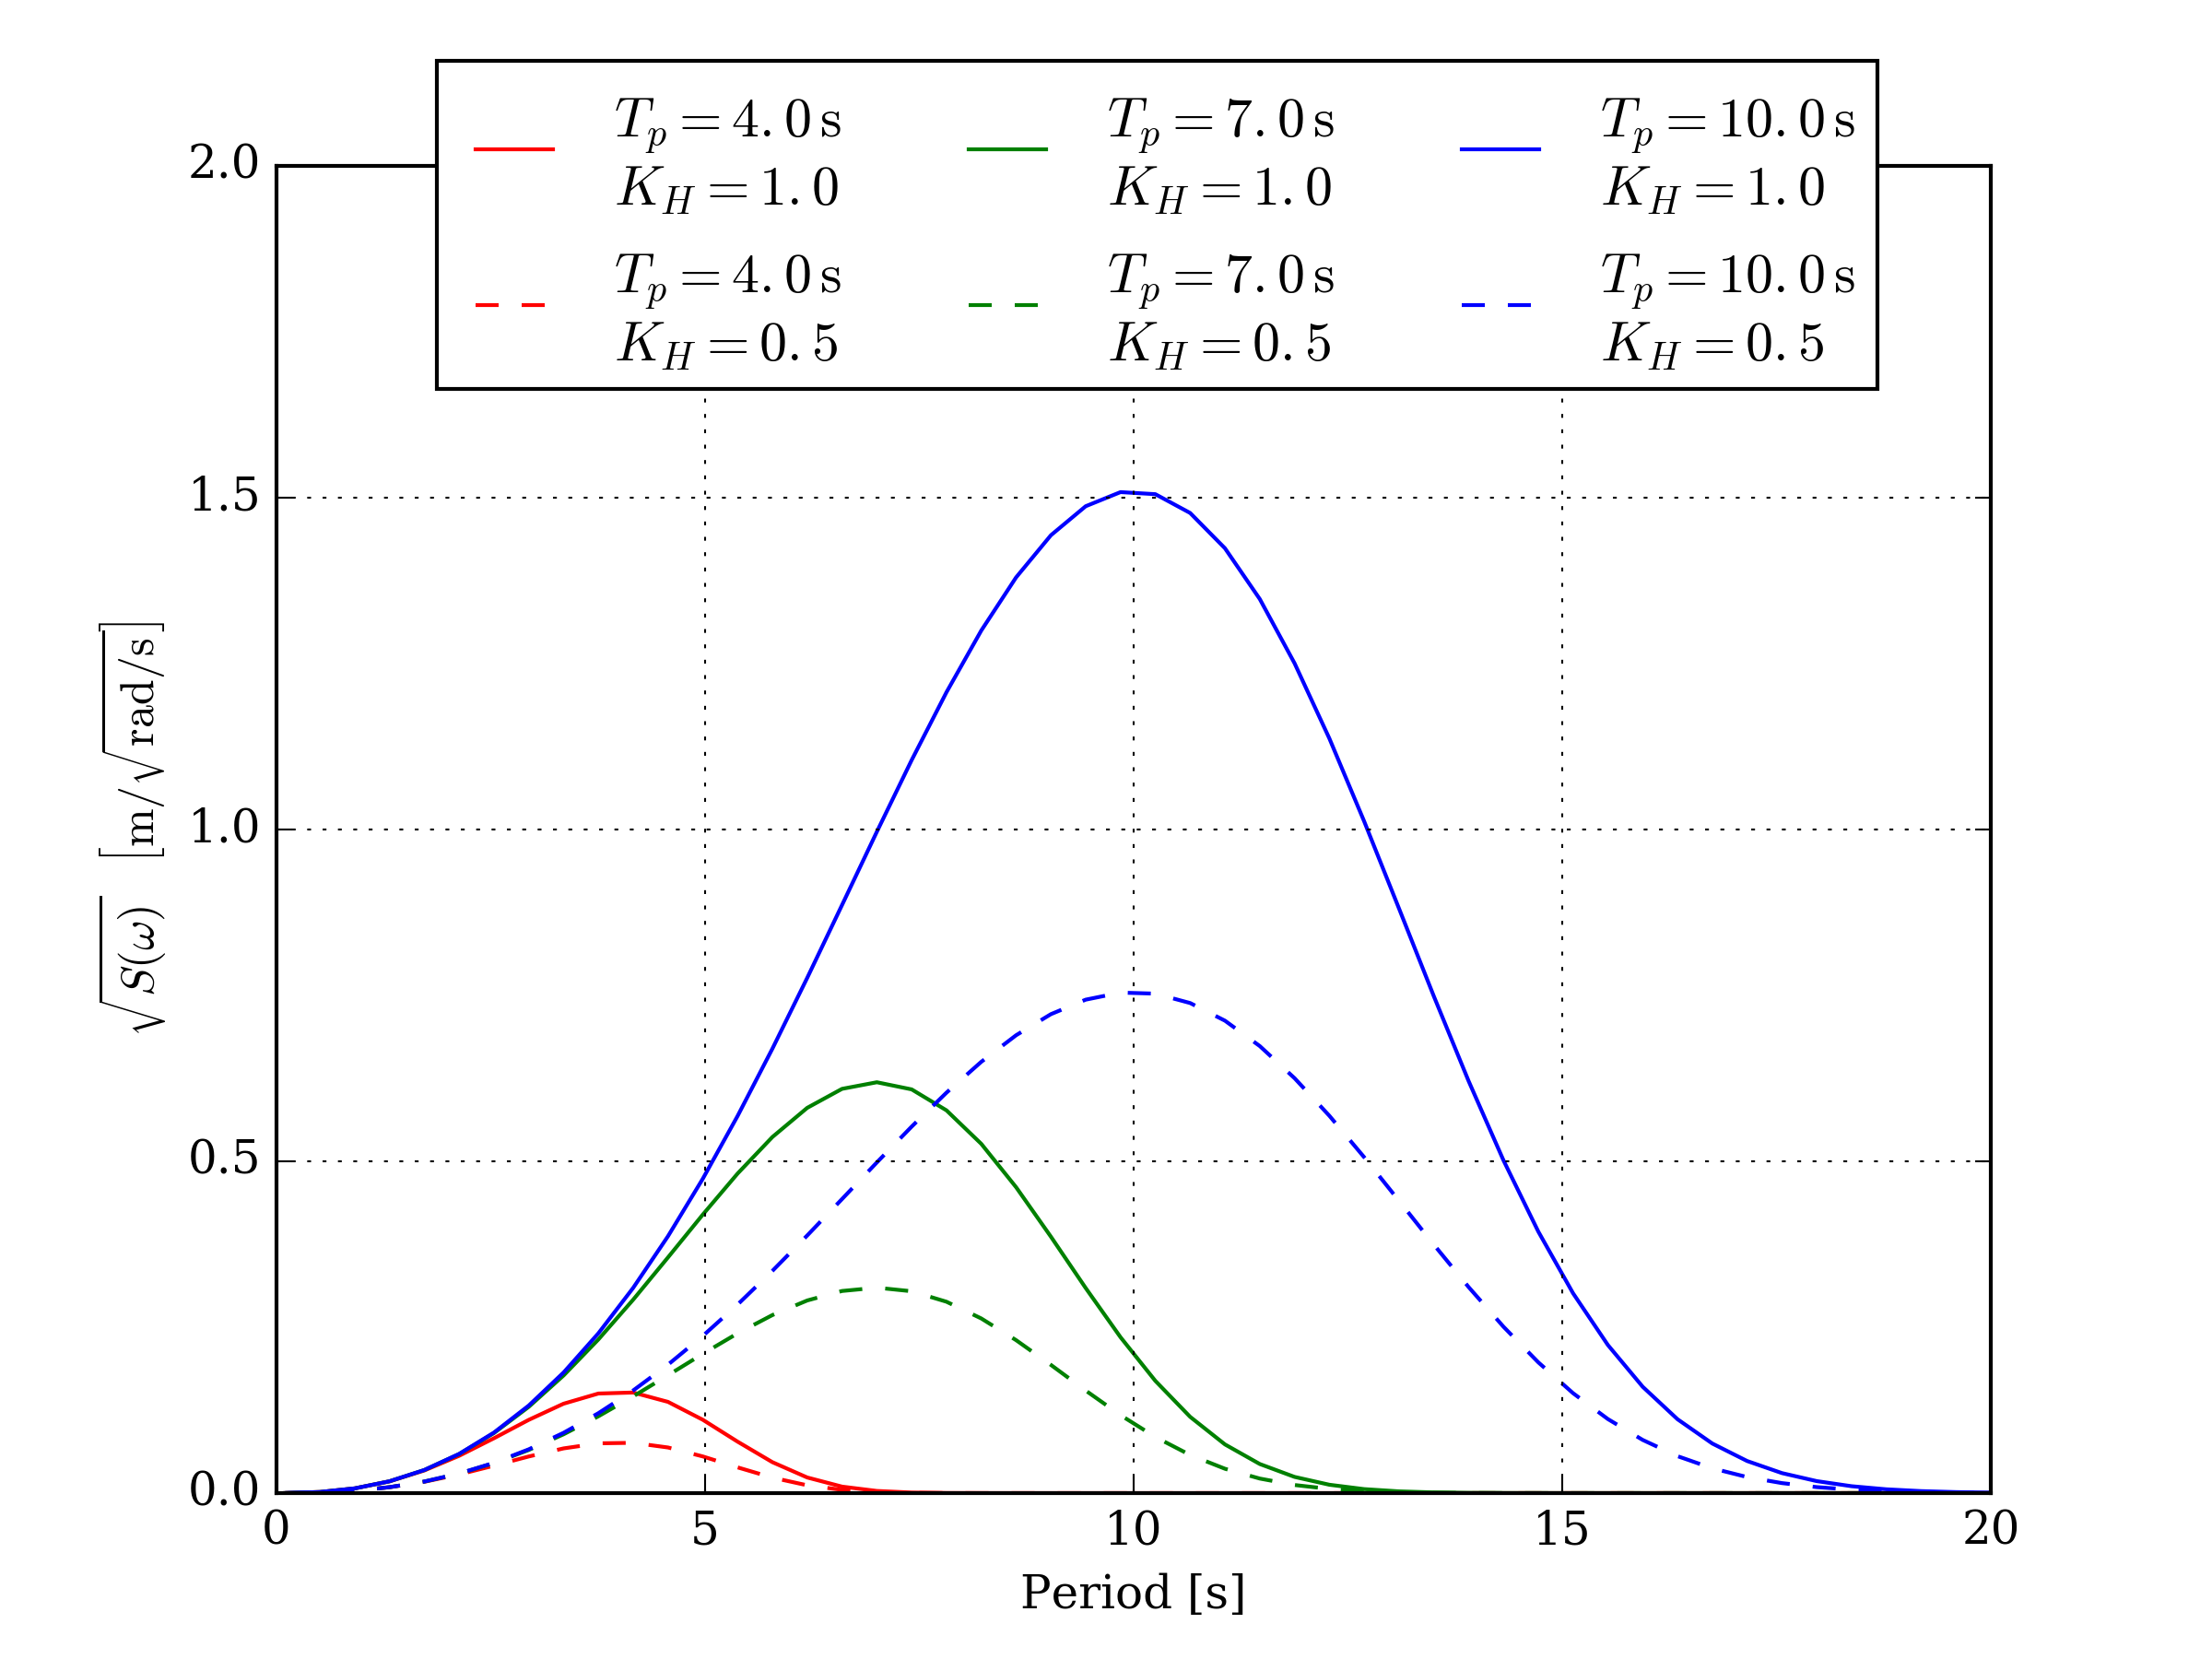
\includegraphics[width=\SFc\textwidth]{images/pm_spectra_2.png}
  \caption{Two-parameter Pierson-Moskowitz wave spectrum shown as a function of wave period for a series of peak period ($T_pz$) values, using two different wave height gains ($K_H$).}
  \label{f:pm}
\end{figure} 
Once the spectrum is defined, the individual wave amplitude values are determined by sampling the wave spectrum according to \eqref{e:amp}.

\subsubsection{Directional Spectra}
For modeling the direction of wave components within the wave field we follow the general approach described by \citet{frechot06realistic}, but improve the method by pre-calculating the relationship between wave characteristics (period, frequency, etc.) and directionality in order to reduce the computational demands of the simulation.

The direction of wave travel can be taken into account using the directional wave spectrum expressed as
\begin{equation}
  E(\omega,\theta)=G(\omega)D(\omega,\theta)
\end{equation}
where $\theta$ represents the wave direction and $D(\omega,\theta)$ is the directional spreading function. %defined such that
%\begin{equation}
%  \int_{-\pi}^{\pi}E(\omega,\theta)d\theta = G(\omega)
%\end{equation}
%for all values of $\omega$.  

The form of $D(\omega,\theta)$ is based on the empirical relations that were proposed by \citet{mitsuyasu75observations}.  The directionality is a function of the normalized frequency $\bar{\omega}=\omega/\omega_p$ and can be expressed as a function of the difference between the angle and the mean angle, $\Delta\theta = \theta_m-\theta$.  The directionality function is then
\begin{equation}
D(\bar{\omega},\Delta\theta) = N(s(\bar{\omega})) \cos{(\Delta\theta/2)}^{2s(\bar{\omega})}
\end{equation}
where the normalizing function
\begin{equation}
N(s(\bar{\omega})) = \left(\frac{1}{2\sqrt{\pi}}\right) \frac{\Gamma(s(\bar{\omega})+1)}{\Gamma(s(\bar{\omega})+1/2)}
\end{equation}
uses the gamma function $\Gamma()$ and the function
\begin{equation}
s(\bar{\omega}) = \left\{
\begin{array}{ll}
  17.01 \, \bar{\omega}^5 \,\, & \mathrm{if} \, \omega \leq \omega_p \\
  17.01 \, \bar{\omega}^{-2.5}  \,\, & \mathrm{if} \, \omega > \omega_p
\end{array}
\right. .
\end{equation}
The shape of the directionality depends upon the component frequency. Spectral components near the peak frequency contain the majority of the wave energy and have a more narrow directional distribution, tending to travel in the mean direction.  Spectral components on either side of the peak frequency tend to have larger variation in direction of travel, in particular lower frequency (longer period) components have a wider distribution of directions than high frequency (shorter period) components.  

To characterize the width of the directional spreading function we use the second moment
\begin{equation}
\mu_2(\bar{\omega}) = \int_{-\pi}^{\pi}(\Delta\theta)^2 D(\bar{\omega},\Delta\theta) d(\Delta\theta)
\end{equation}
which we evaluate numerically. This relationship is pre-computed and used as a lookup table for the component waves which make up the wave field.  For each wave component in \eqref{e:gerstner} the direction of the wavevector is determined by the user-specified mean direction and an additional random direction component.  This additional component is generated as a sample from a zero mean, normal distribution with a variance set equal to $\mu_2(\bar{\omega})$.  


\subsection{Wind Modeling}\label{s:wind_model}
Wind is a significant disturbance for objects at the sea surface. We consider the total wind speed $V_w(t)$ consisting of the sum of the constant mean wind speed ($\bar{v}$) and stochastic, zero-mean, variable wind speed ($v_g(t)$) due to turbulence and gusting, i.e., $V_w(t)=\bar{v}+v_g(t)$.

Spectral representations of ocean wind environments are common and generally model the variable component of wind speed as a wide-sense stationary, Gaussian stochastic process.  Typical models of wind over water include \citet{harris71nature}, \citet{forristall88wind} and \citet{ochi13wind}. \citet{cole18reactive} showed that the Forristall and Ochi and Shin models are in agreement, while the Harris model underestimates the spectral content.  While the implementation is not specific to any one spectral model of stochastic wind, for illustration purposes we use the Forristall wind spectra.  The form of the one-sided spectra is \citet{olesen84modelling} blunt model for micrometeorology, where Forristall showed that normalizing the one-sided spectrum by the variance ($\sigma$) produced improved experimental agreement:
\begin{equation}
  \widetilde{S}_f(f) = \frac{S_f(f)\,f}{\sigma^2}  = \frac{ A f^*}{( 1 + B f^*)^{5/3}}.
    \label{e:forristall}
    \end{equation}
    In this dimensionless form $f$ is the oscillation frequency in \unit[]{Hz} and $f^*$ is the standard nondimenstional frequency from atmospheric boundary layer studies,
\begin{equation}
  f^* = \frac{f \, z}{\bar{v}(z)},
\end{equation}
where $z$ is the height and $\bar{v}(z)$ is the mean wind speed as a function of height. The constants $A$ and $B$ are chosen to fit specific observational data.  We use the mean coefficients from of $A=42.0$ and $B=63.0$, as reported by \citet{forristall88wind}  These values satisfy the constraint $A=(2/3)B$, necessary so that the variance of the stochastic process is $\sigma^2$, i.e.,
\begin{equation}
  \int_0^{\infty} S_f(f) df = \sigma^2.
\end{equation}
The Forristall normalized spectrum is illustrated in Figure~\ref{f:forristall_norm}.   The peak of the spectrum (\ref{e:forristall}) occurs at
\begin{equation}
f^*_p = \frac{3}{2B}.
\end{equation}
%so for a height of $z=\unit[10]{m}$ the dimensional peak frequency increases linearly with wind velocity,
%\begin{equation}
%f_p = \frac{3}{2Bz}\bar{v}_{10}.
%\end{equation}
\begin{figure}[h!]
  \centering
  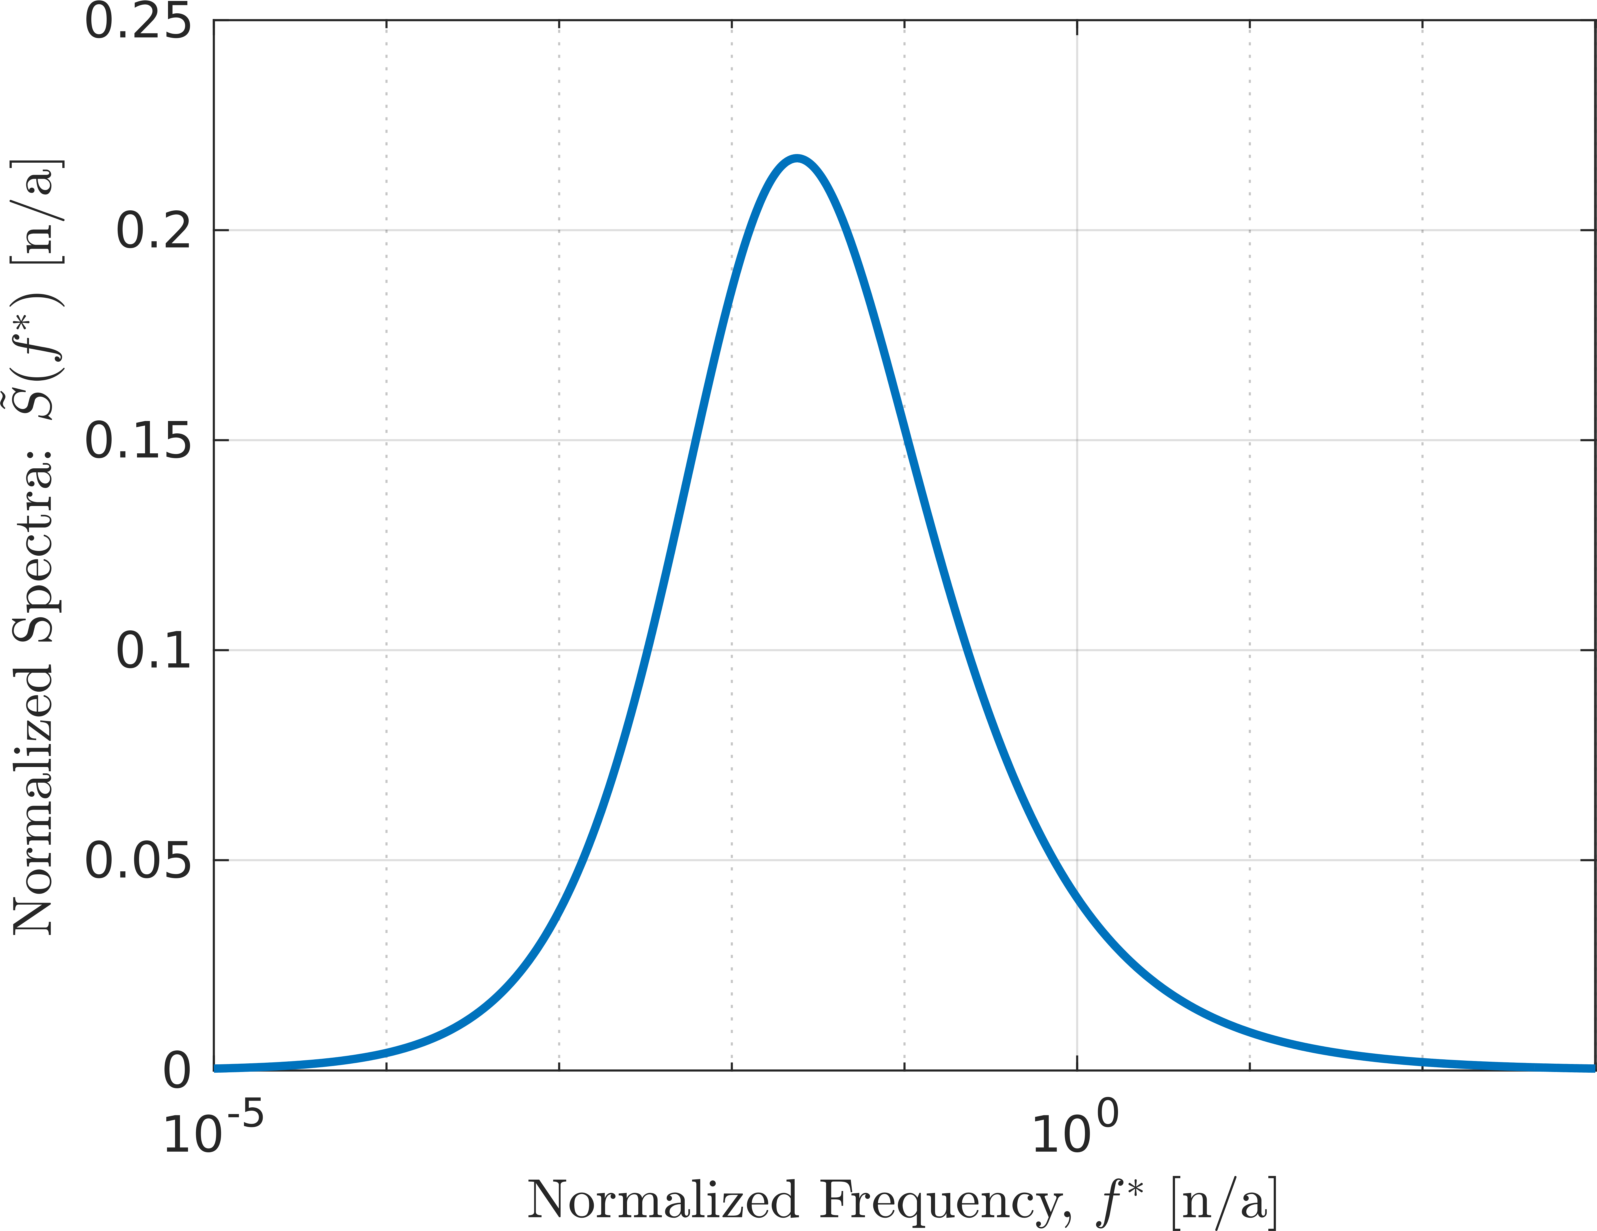
\includegraphics[width=\SFc\textwidth]{forristall_norm.png}
  \caption{Forristall normalized spectrum.}
  \label{f:forristall_norm}
\end{figure}

For generating physically meaningful wind time series simulations it is necessary to take into account the physical dimesions of the spectra.  We consider a constant height of $z=\unit[10]{m}$ and mean wind velocity at that height $\bar{v}(z=10)=\bar{v}_{10}$.  Figure~\ref{f:forristall_dim} illustrates how mean wind speed affects the generated spectra. 
\begin{figure}[hbt!]
  \centering
  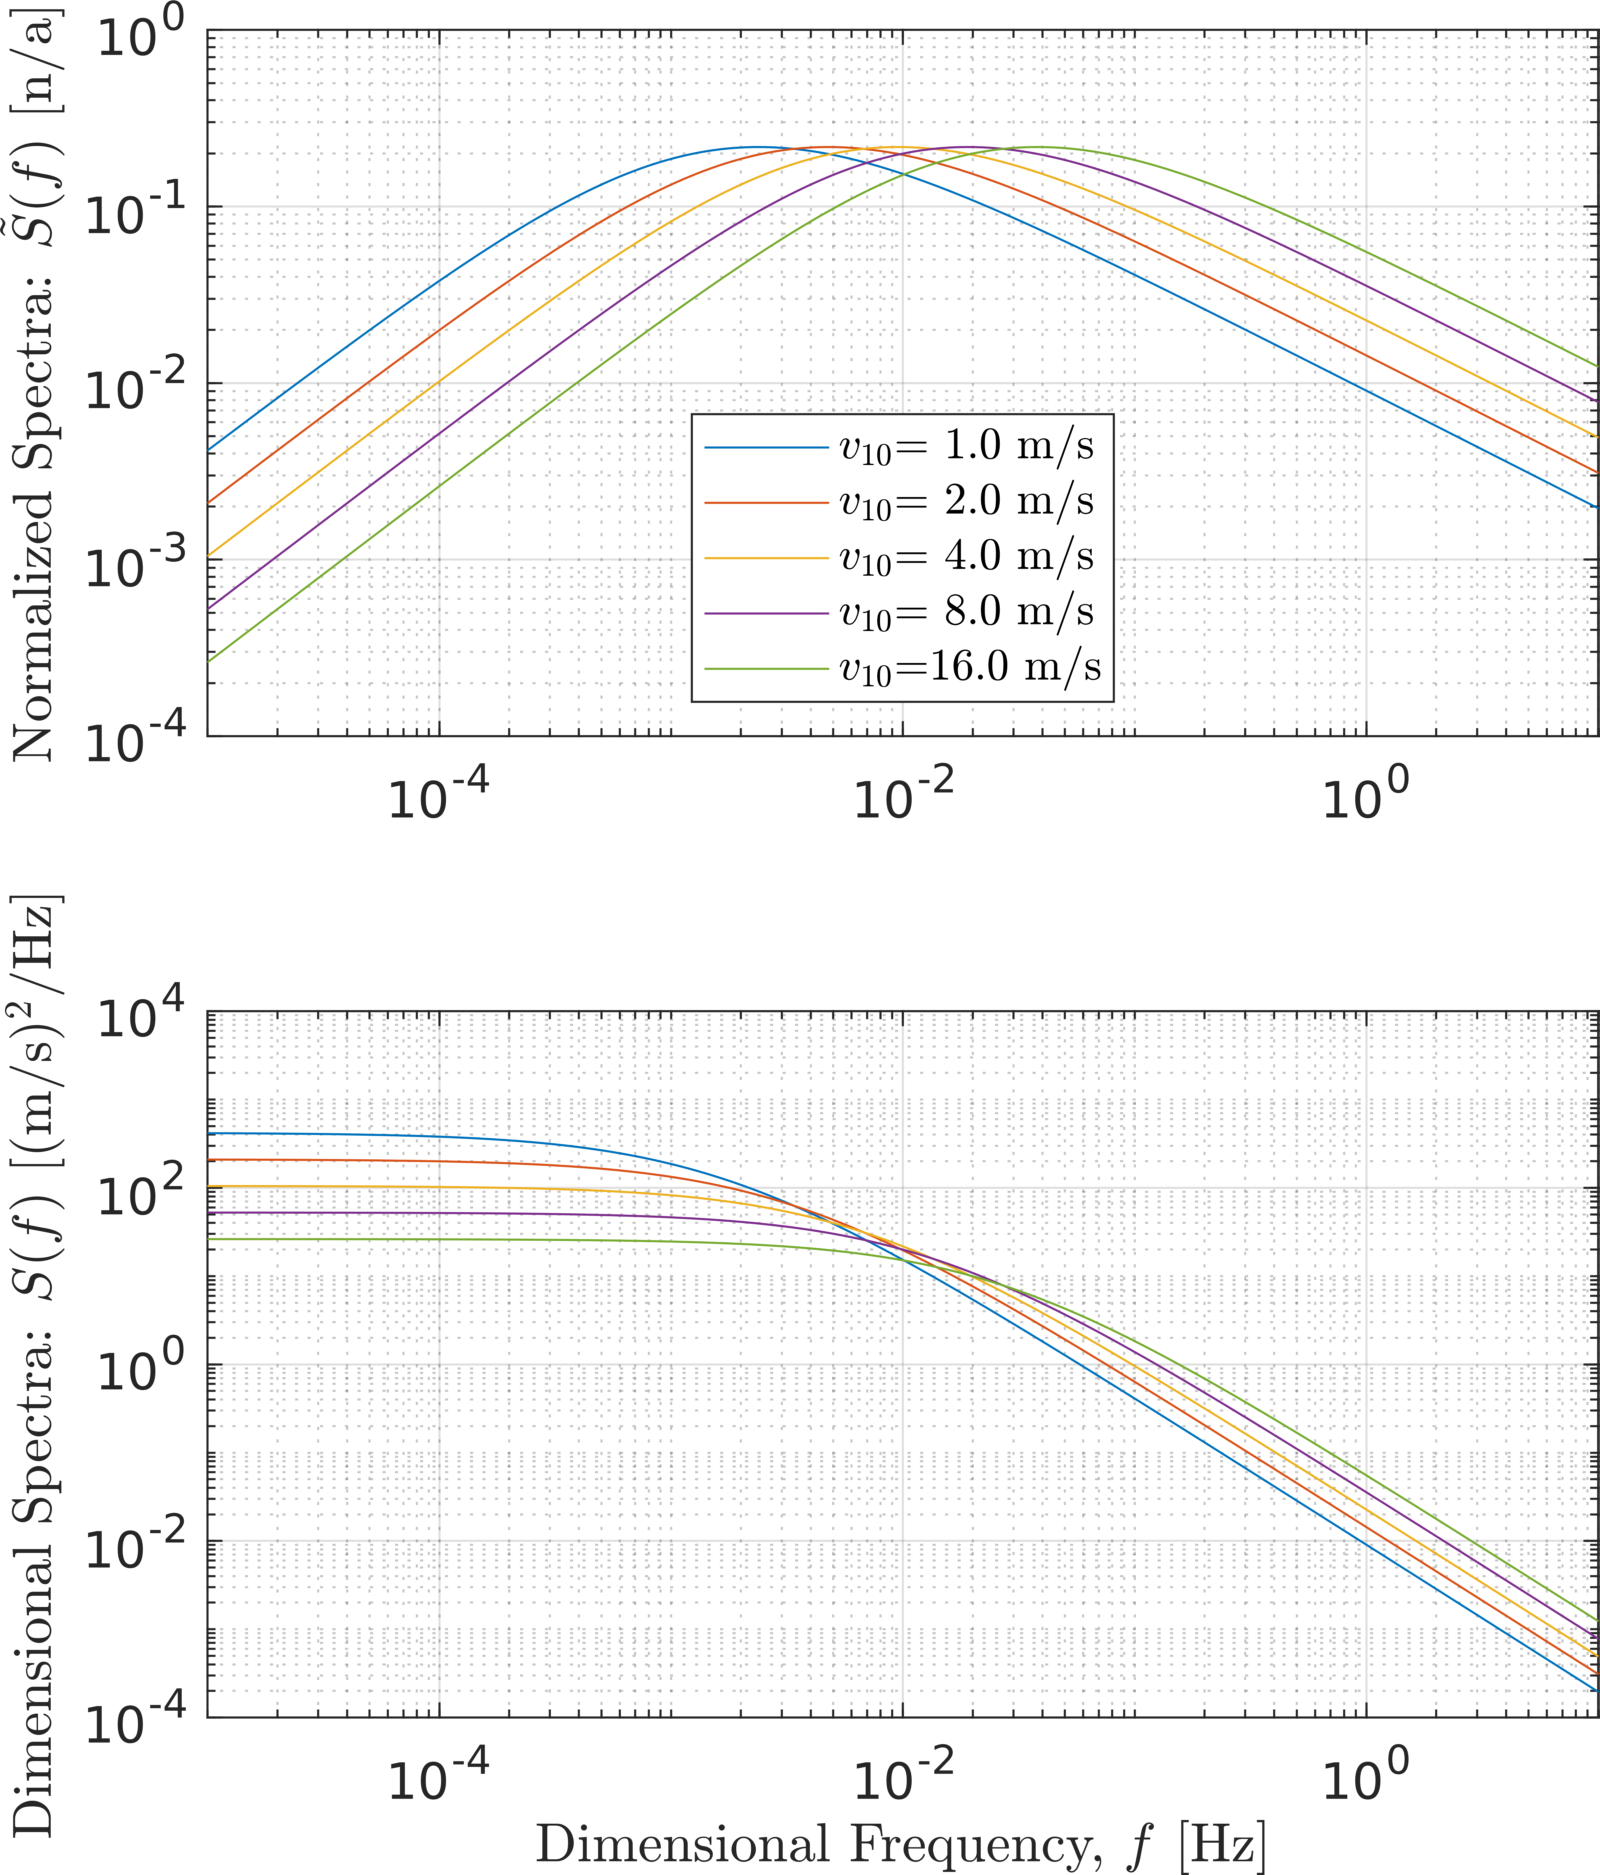
\includegraphics[width=\SFc\textwidth]{forristall_dim.png}
  \caption{Dimensional Forristall spectra with unit variance. }
  \label{f:forristall_dim}
\end{figure}
The cutoff frequency $f_c$ for the dimensional spectra is the frequency for which $S_f(f_c) = 0.5 S_f(0)$.  In dimensionless and dimensional forms, the cutoff frequency is
\begin{IEEEeqnarray}{rCl}\IEEEyesnumber\label{e:cutoff}
  f^*_c & = & \frac{2^{3/5}-1}{B} \\
  f_c & = & \frac{(2^{3/5}-1)\bar{v}(z)}{B\,z} \\
      & = & (\num{8.19e-4}) \, \bar{v}_{10} %\; \mathrm{Hz}.
  \end{IEEEeqnarray}

\subsubsection{Wind speed variance}
In the Forristall model the variance of the wind speed is not a simple function of the mean wind speed.  The ratio of the variance to the friction velocity ($v_*$) can be approximated as
\begin{equation}
\frac{\sigma}{v_*} = 3.0 w
\label{e:sigratio}
\end{equation}
where $w$ is determined from the predicted ocean significant wave height $H_n$ and the observed significant wave height $H_s$ as
\begin{equation}
w = 1 + \frac{H_s-H_n}{2 H_n}.
\label{e:wavefactor}
\end{equation}
For the purposes of this example, we consider a developed sea where $H_s=H_n$.

The friction velocity is determined by using the logarithmic boundary layer mean velocity profile
\begin{equation}
\bar{v}(z) = \frac{v_*}{\kappa}\ln{\left(\frac{z}{z_0}\right)}
\label{e:profile}
\end{equation}
where the von Karman's constant is $\kappa=0.41$ and $z_0$ is the sea surface roughness.  It is common to re-write (\ref{e:profile}) at a reference altitude of $z=\unit[10]{m}$ and solve for the friction velocity
\begin{equation}
v_* = \frac{\kappa \, \bar{v}(z=10)}{\ln(z=10/z_0)} = \frac{\kappa \, \bar{v}_{10}}{\ln(10/z_0)}.
\label{e:profile10}
\end{equation}
Multiple models of the relationship between sea surface roughness ($z_0$) and friction velocity ($v_*$) are available.  Based on dimensional analysis \citet{charnock55wind} proposed 
\begin{equation}
\frac{z_0 g }{v_*^2} = \alpha
\label{e:charnock}
\end{equation}
where $g$ is the acceleration of gravity; $\alpha = [0.013, 0.0185]$ has been found to be consistent with empirical wind profiles over the ocean \citep{garratt77review,toba90wave}.  %Alternatively this relationship can be considered to be a function of the degree of wave development, or wave age,
%\begin{equation}
%\frac{z_0 g }{v_*^2} = \mathsf{f} (c_p/v_*)
%\label{e:waveage}
%\end{equation}
%where $c_p$ is the phase velocity of the dominant wave and $c_p/v_*$ describes wave age \citep{myrhaung09effect}.  An example of the functional relationship for (\ref{e:waveage}) is provided in \citep{volkov01dependence}.

Without loss of generality, we numerically solve for $V_{*}$ by combining (\ref{e:profile10}) and (\ref{e:charnock}) with $\alpha= 0.0144$ for values of $v_{10} = [4, 21]\unit[]{m/s}$ \citep{garratt77review}.  The resulting values are illustrated in Figure~\ref{f:wind_consts}.
\begin{figure}[hbt!]
  \centering
  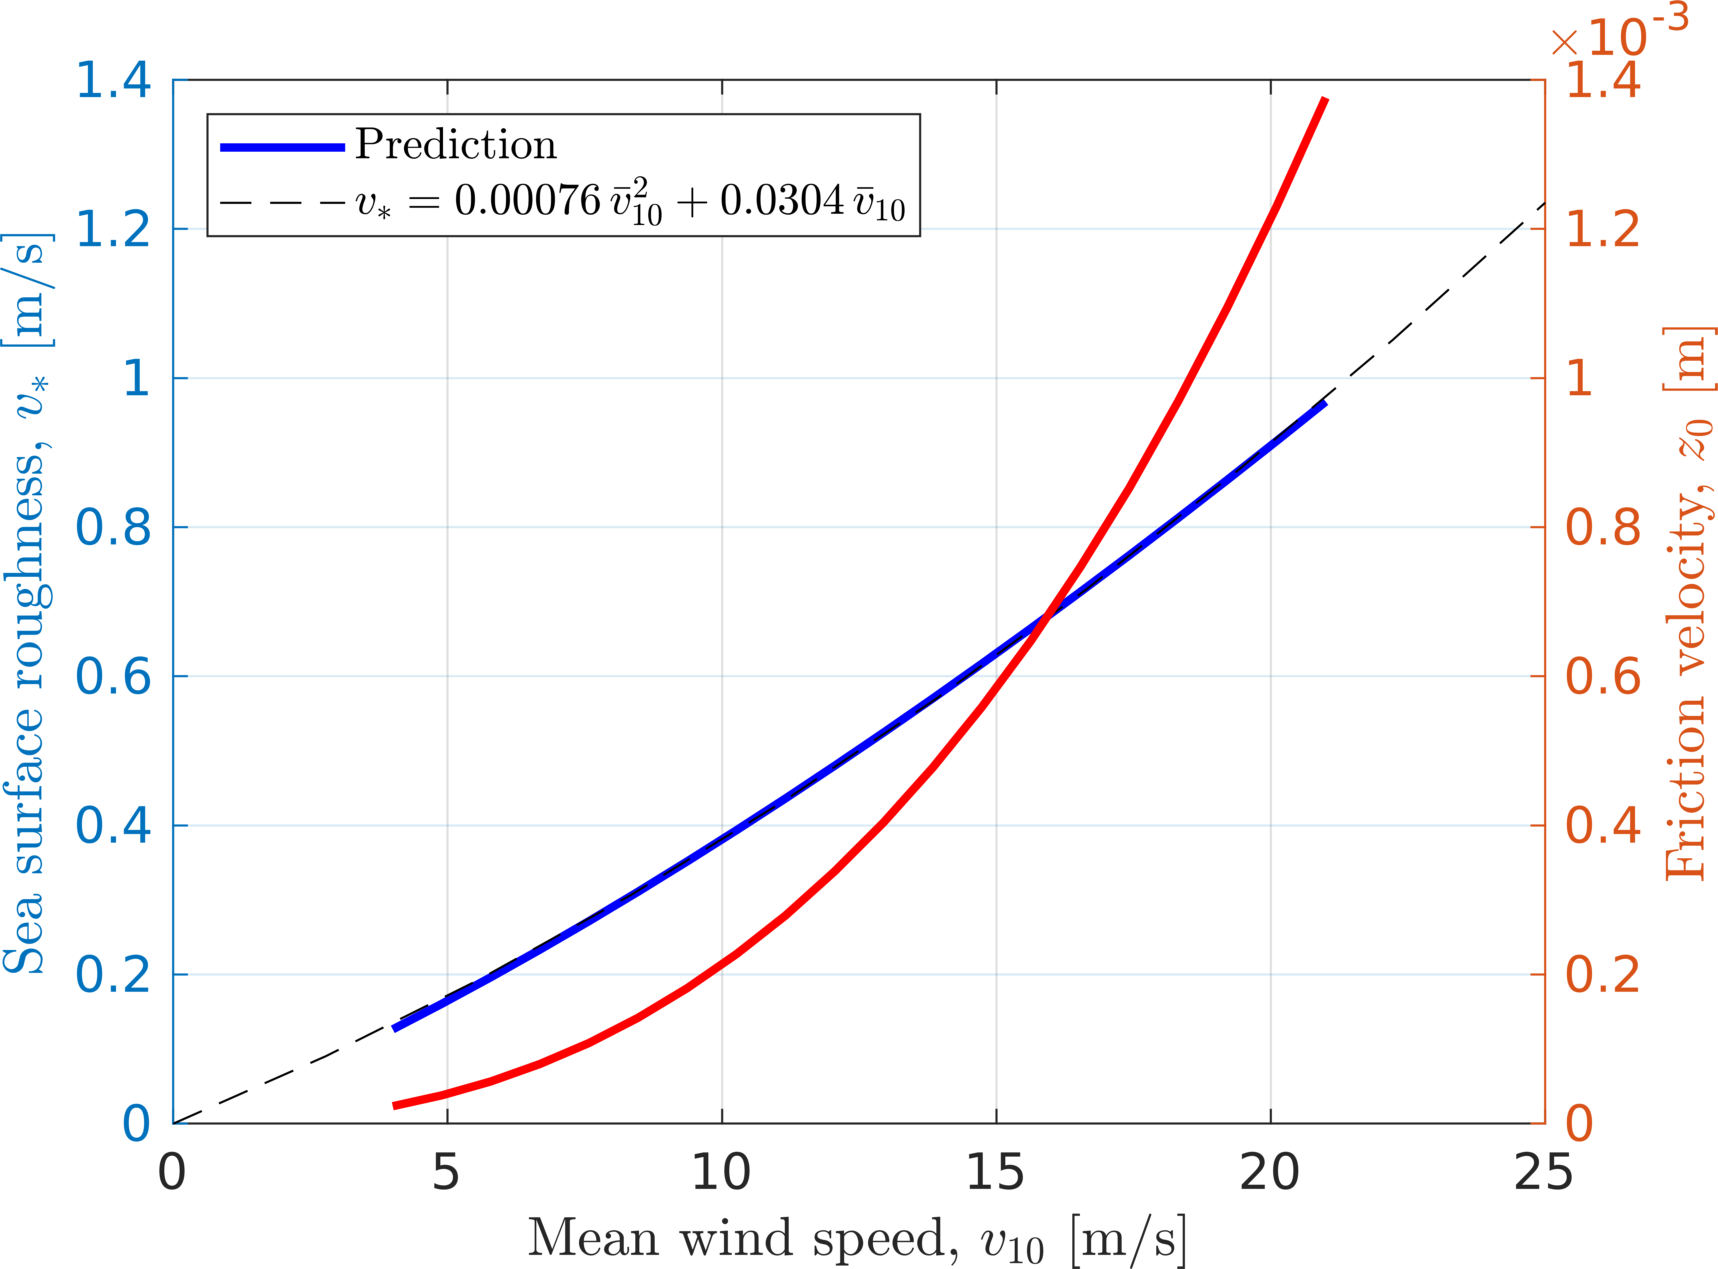
\includegraphics[width=\SFc\textwidth]{wind_consts.png}
  \caption{Sea surface roughness and friction velocity as a function of mean wind speed.}
  \label{f:wind_consts}
\end{figure}
To simplify the implementation, we fit a quadratic polynomial to the sea surface roughness prediction via nonlinear regression, enforcing that the y-intercept be zero.  The resulting relationship, also shown in Figure~\ref{f:wind_consts}, is
\begin{equation}
v_* = 0.00076 \, \bar{v}_{10}^2 + 0.0304 \, \bar{v}_{10}
\label{e:fit}
\end{equation}
which allows expression of the wind speed variance as a function of mean wind speed,
\begin{equation}
\sigma^2 = \left[ 3 \, w (0.00076 \, \bar{v}_{10}^2 + 0.0304 \, \bar{v}_{10})\right]^2.
\label{e:fit2}
\end{equation}
Substituting (\ref{e:forristall}) and the constants described above into (\ref{e:fit2})  allows us to express the dimensional Forristall spectrum for wind speed at $z=\unit[10.0]{m}$ altitude as a function of only the mean wind speed,
\begin{multline}
S_f(f) =  \left[ 3 \, (0.00076 \, \bar{v}_{10}^2 + 0.0304 \, \bar{v}_{10})\right]^2 \\
\frac{(42.0)10.0/\bar{v}_{10}}{\left(1+\frac{63.0 (10.0) f}{\bar{v}_{10}}\right)^{5/3}}.
\label{e:dimensional}
\end{multline}

\vspace{3em}

\subsubsection{Generating Wind Time Series}
The wind model is described by the PSD in (\ref{e:dimensional}) which allows us to generate sample functions of the underlying stochastic process using a summation of cosines approach similar to the implementation of the Gerstner waves.  The combined turbulence and gusting wind speed is expressed as
\begin{equation}
  v_g(t) = \sqrt{2} \sum_{n=0}^{M-1} A_n \cos(\omega_n t + \phi_n)
  \label{e:sumcosines}
\end{equation}
where
\begin{IEEEeqnarray}{C}
\IEEEyesnumber\label{e:sim2} \IEEEyessubnumber*
A_n = \left(\frac{1}{2 \pi} S_{f}(f_n = \omega_n / (2 \pi)) \Delta \omega\right)^{1/2},  \label{e:an} \\
\omega_n = n \Delta \omega, \; n=0,1,2,...,N-1 \label{e:lrs2}\\
\Delta \omega = \omega_u / M.
\end{IEEEeqnarray}
The frequency sampling is $\Delta\omega$, the upper cut-off frequency, $\omega_u$, is the frequency beyond which the PSD may be assumed to be zero, $\phi_0, \phi_1, ... , \phi_{M-1}$ are random phase angles distributed uniformly over the interval $[0,2\pi)$.  Note the factor of $1/(2\pi)$ in (\ref{e:an}) is necessary to maintain the integral relationship between the spectrum and the variance of the underlying stochastic process, i.e.,
\begin{IEEEeqnarray}{rcl}
\IEEEyesnumber\label{e:freq} \IEEEyessubnumber*
E[v_g^2(t)] & = & \sigma_{v_g}^2 \\
& = &\int_{0}^{\infty}S_{f}(f)df \\
& = &\frac{1}{2\pi}\int_{0}^{\infty}S_{f}(f=\frac{\omega}{2\pi}) d\omega \\
& \leq & \frac{1}{2} \left( \frac{2 \pi}{\Delta \omega} \right) \frac{1}{M}.
\end{IEEEeqnarray}
The condition
\begin{equation}
  A_0 = 0 \; \mathrm{or} \; S_{f}(\omega_0=0)=0
  \label{e:an0}
\end{equation}
is necessary and must be forced if $S_{yy}(0)\neq 0$.  The resulting simulated time series is periodic with period
\begin{equation}
  \label{e:T0}
  T_0 = \frac{2\pi}{\Delta \omega}.
\end{equation}

By combining (\ref{e:dimensional}), (\ref{e:sumcosines}) and (\ref{e:sim2}) we are able to generate a physically relevant time series realization, $v_g$, of the variable wind speed stochastic process described by the Forristall wind spectrum.  For wind at $z=0$ and a fully developed sea ($H_s=H_n$) this time series is solely a function of mean wind speed, $\bar{v}=v_{10}$. The example in Figure~\ref{f:forristall} illustrates the results for three different mean wind speeds.
\begin{figure}[h!]
  \centering
  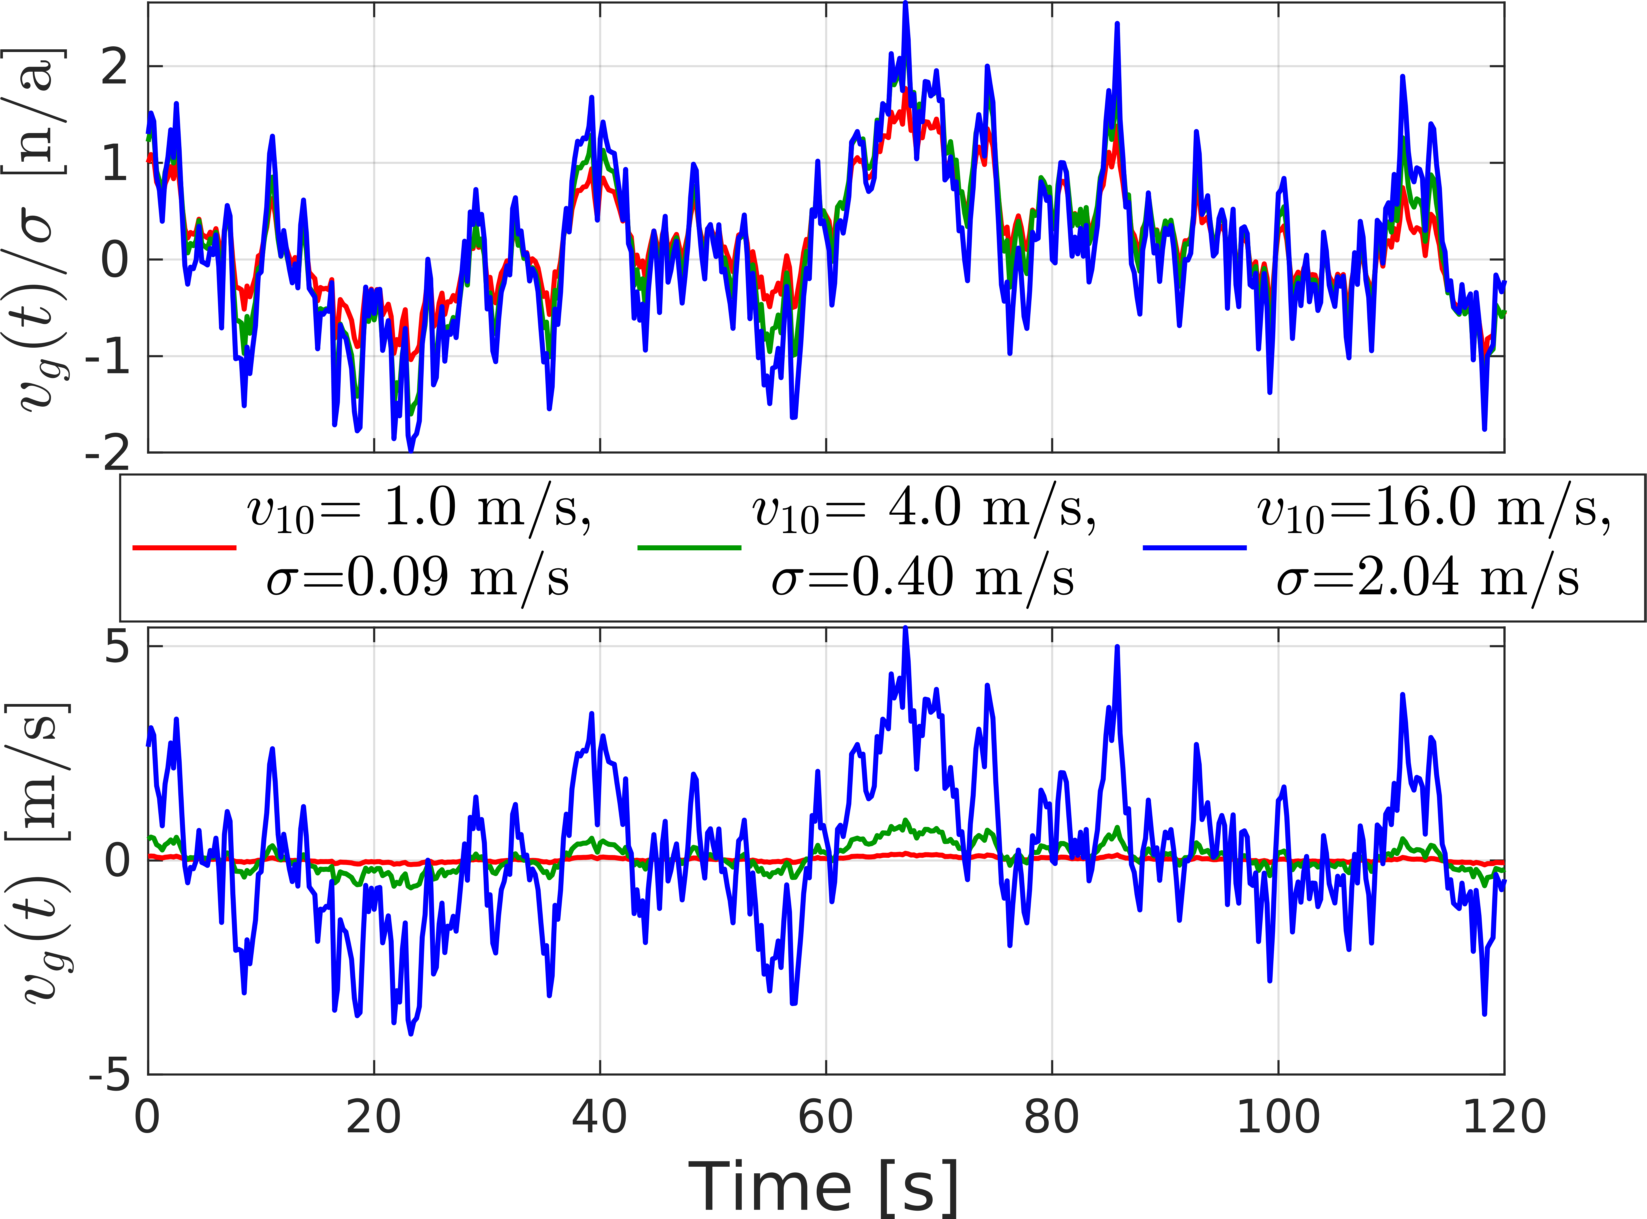
\includegraphics[width=\SFc\textwidth]{src/foristall_time_ex.png}
  \caption{Example time series of variable wind speed component generated by spectral representation for Forristall spectrum for different mean wind speed values.}
  \label{f:forristall}
\end{figure}
In the upper axis, the speed is normalized by the standard deviation of the time series to illustrate the similarity in the results. This view also highlights that the higher mean wind velocities generate spectra with a slightly higher cutoff frequency (\ref{e:cutoff}).
%
\section{Vehicle Model}
%
To approximate the motion of a surface vehicle in the ocean environment, we adapt the six degree-of-freedom robot-like vectorial model for marine craft, proposed by \citet{fossen11handbook}, and expressed as\footnote{The rigid-body terms can be expressed equivalently using either the total vessel velocity or the velocity relative the the fluid, see Property 8.1 of \citet{fossen11handbook}.  For our implementation the rigid-body terms and the hydrodynamics terms are solved for separately, and it is more direct to leverage the native physics engine in terms of total rigid-body velocity.}
\begin{equation}
\begin{split}
&\underbrace{\bm{M}_{RB}\dot{\bm{\nu}}+\bm{C}_{RB}(\bm{\nu})\bm{\nu}}_\text{rigid-body forces} + \\
&\underbrace{\bm{M}_A\dot{\bm{\nu}}_r + \bm{C}_A(\bm{\nu}_r)\bm{\nu}_r + 
  \bm{D}(\bm{\nu}_r)\bm{\nu}_r}_\text{hydrodynamic forces} + 
\underbrace{\bm{g}(\bm{\eta})}_\text{hydrostatic forces} \\
& = \bm{\tau}_{propulsion}+\bm{\tau}_{wind}+\bm{\tau}_{waves}
\label{e:fossenmodel}
\end{split}
\end{equation}
where
\begin{IEEEeqnarray}{rCl}\IEEEyesnumber\label{e:estate}
    \bm{\eta} & = & [x, y, z, \phi, \theta, \psi]^T \IEEEyessubnumber \\
    \bm{\nu}  & = & [u, v, w, p, q, r]^T \IEEEyessubnumber
\end{IEEEeqnarray}
are the position and velocity vectors respectively for surge, sway, heave, roll, pitch and yaw.  The total velocity, $\bm{\nu}$, is the sum of an irrotational water current velocity, $\bm{\nu}_c$, and the vessel velocity relative to the fluid, $\bm{\nu}_r$, i.e., $\bm{\nu}=\bm{\nu}_r+\bm{\nu}_c$.  The forces and moments due to propulsion (control), wind, and waves are represented as $\bm{\tau}_{propulsion}$, $\bm{\tau}_{wind}$ and $\bm{\tau}_{waves}$.

Traditionally, surface vessel models are separated into \emph{maneuvering} models (representing the surge, sway and yaw degrees-of-freedom) and \emph{seakeeping} models (representing the heave, pitch and roll degrees-of-freedom). For the purposes of supporting the development of autonomy, it is important that the unified simulation model include \emph{both} maneuvering and seakeeping degrees-of-freedom. The maneuvering aspects of the model influence the vessel steering and control portion of the autonomy solution. The inclusion of the seakeeping aspect of the model is critical for exercising the sensory perception portion of the autonomy solution.

Our approach to formulating both portions of our unified model is identical. We seek the lowest fidelity representation possible for each that is able to achieve the correct type of dynamic response but not necessarily the correct magnitude of that particular response. For a maneuvering surface vessel, the hydrodynamic terms, particularly the damping terms, play a critical role in the type of resultant motion \color{red} since the hydrostatic terms do not act in the horizontal plane. On the other hand, the seakeeping degrees-of-freedom are dominated by the hydrostatic and wave excitation forces. Even without nondiagonal added-mass and nonlinear damping terms in these degrees-of-freedom, the vehicle model still produces oscillatory motion which induces sensor changes that can impact perception. By neglecting these terms, our model will typically produce larger motion responses, but it will not change the kind of response the simulation produces. For example, the lack of a nonlinear damping term for the roll degree of freedom will potentially result in overly large roll angles in response to wave encounters, but the dominant restoring moment from the hydrostatic term is present.\color{black}

Our intended use of the VRX simulation, as described in this article, does not justify the additional complexity and challenges associated with incorporating the neglected hydrodynamic terms into either portion of our unified model. Finally, it is important to note that the unified model formulation presented here is intended for a small unmanned surface vehicle. When modeling different vehicles, such as unmanned underwater vehicles, the model may need to be altered to include additional hydrodynamic terms. This would dependent on the specific vehicle geometry and any appendages it contained.%
%The motion of a vessel is approximated in simulation by estimating each of the constituent forces in \eqref{e:fossenmodel} at each time step of the simulation. The rigid body components are simulated using the Gazebo physics engine.  The remaining constituents are simulated using the model components described below.
%
\subsection{Hydrodynamic Forces}\label{s:hydro}
%
The hydrodynamic forces in \eqref{e:fossenmodel} include the added mass terms due to the inertia of the surrounding fluid and hydrodynamic damping terms due to the vehicle interacting with the surrounding fluid. The terms a captured using coefficients, typically referred to as hydrodynamic derivatives, and expressed using SNAME (1950) notation \citep{fossen11handbook}.

\color{red}The added mass matrix for our vehicle model is expressed as
\begin{equation}\hspace{-0.15in}
\medmath{
\bm{M}_{A}= -\left[ 
\begin{array}{cccccc}
X_{\dot{u}} & 0 & 0 & 0 & 0 & 0 \\
0 & Y_{\dot{v}} & 0 & 0 & 0 & Y_{\dot{r}} \\
0 & 0  &Z_{\dot{w}} & 0 & 0 & 0 \\
0 & 0 & 0 &K_{\dot{p}} & 0 & 0 \\
0 & 0 & 0 & 0 &M_{\dot{q}} & 0 \\
0 & N_{\dot{v}} & 0 & 0 & 0 & N_{\dot{r}} 
\end{array} \right]
}
\end{equation}
where, according to \citet{fossen11handbook} we can assume $N_{\dot{v}} = Y_{\dot{r}}$ for the \wamv{} since it is a slow moving surface ship.

The surge, sway, yaw components of our model match the maneuvering model used by \citet{sarda16station}. For the heave, roll, pitch components, we follow the six degree-of-freedom coupled motion manuevering model presented by \citet{fossen11handbook} that only contains the diagonal terms for these components. As noted by \citet{fossen11handbook}, the off-diagonal elements of the added mass matrix, $\bm{M}_{A}$ will be small compared to the diagonal elements for most hullforms.


Once the added mass terms to include in the model that make up $\bm{M}_{A}$ are chosen, the derivation by \citet{imlay61complete} provides the Coriolis-centripetal added mass terms that result. The Coriolis-centripetal added mass matrix is expressed using the same hydrodynamic derivatives from $\bm{M}_{A}$. The resultant matrix is
\begin{multline}% ***need to fix formatting of matrix to stop spillage
    \medmath{\bm{C}_{A}(\bm{\nu}_r)=
    \left[ 
    \begin{array}{ccc}
        0 & 0 & 0 \\
        0 & 0 & 0 \\
        0 & 0 & 0 \\
        0 & -Z_{\dot{w}}w_r & Y_{\dot{v}}v_r \\
        -Z_{\dot{w}}w_r & 0 & -X_{\dot{u}}u_r \\
        -Y_{\dot{v}}v_r - Y_{\dot{r}}r & X_{\dot{u}}u_r & 0 
    \end{array}
    \right.}
    \\
    \medmath{
    \left. 
    \begin{array}{ccc}
        0 & -Z_{\dot{w}}w_r & Y_{\dot{v}}v_r+Y_{\dot{r}}r \\
        Z_{\dot{w}}w_r & 0 & -X_{\dot{u}}u_r\\
        -Y_{\dot{v}}v_r & X_{\dot{u}}u_r & 0 \\
        0 & -N_{\dot{r}}r_r & M_{\dot{q}}q_r \\
        N_{\dot{r}}r_r & 0 & -K_{\dot{p}}p_r \\
        -M_{\dot{q}}q_r & K_{\dot{p}}p_r & 0 
    \end{array}
    \right].}
\end{multline}

Since the terms of the maneuvering portion of our unified model are chosen to match those of \citet{sarda16station}, we simply used their theoretical expressions to estimate the values for $X_{\dot{u}}$, $Y_{\dot{v}}$, $N_{\dot{r}}$, and $Y_{\dot{r}}$. To estimate the added mass terms in the seakeeping portion of our model we used the previous work of \citet{greenhow88added} involving the study of added mass and damping of partially submerged horizontal cylinders in heave and sway. From their work we were able to directly estimate the heave added mass, $Z_{\dot{w}}$, by assuming that each pontoon could be represented by a circular cylinder. For the roll and pitch added mass, we assumed that half of this added mass acted at half the beam, for roll, and a quarter of the length, for pitch.\color{black}

The hydrodynamic damping includes forces due to radiation-induced potential damping, skin friction, wave drift damping, vortex shedding and lifting forces \citep{fossen11handbook,krishnamurthy05modeling}.  These effects are aggregated in the hydrodynamic damping matrix 
\begin{equation}
\bm{D}(\bm{\nu}_r) = \bm{D}_l+\bm{D}_n(\bm{\nu}_r)
\end{equation}
expressed as a sum of linear and quadratic terms:
\begin{equation}
  \medmath{
\bm{D}_l= -\left[ 
\begin{array}{cccccc}
X_{u} & 0     & 0     & 0     & 0     & 0\\
0     & Y_{v} & 0     & 0     & 0     & Y_{r}\\
0     & 0     & Z_{w} & 0     & 0     & 0 \\
0     & 0     & 0     & K_{p} & 0     & 0 \\
0     & 0     & 0     & 0     & M_{q} & 0 \\
0     & N_{v} & 0     & 0     & 0     & N_{r}
\end{array} \right]
}
\label{e:D}
\end{equation}
and
\begin{multline}\label{e:D_n}
  \medmath{
    \bm{D}_n(\bm{\nu}_r) =
  }
  \\
  \medmath{
    -\left[ 
      \begin{array}{cccccc}% *** did an ad-hoc horizontal spacing fix here; perhaps there's a more elegant solution
          X_{u|u|}|u_r| & \hspace{-0.25in}0 & 0 & 0 & 0 & \hspace{-0.10in}0 \\
          0 & \hspace{-0.25in}Y_{v|v|}|v_r| & 0 & 0 & 0 & \hspace{-0.10in}0  \\
          0 & \hspace{-0.25in}0 & 0 & 0 & 0 & \hspace{-0.10in}0   \\
          0 & \hspace{-0.25in}0 & 0 & 0 & 0 & \hspace{-0.10in}0  \\
          0 & \hspace{-0.25in}0 & 0 & 0 & 0 & \hspace{-0.10in}0  \\
          0 & \hspace{-0.25in}0 & 0 & 0 & 0 & \hspace{-0.10in}N_{r|r|}|r| 
      \end{array} \right].
  }
\end{multline}

\color{red} As discussed in \citet{fossen11handbook}, for a surface vehicle, the linear damping matrix captures predominately two effects, viscous skin-friction damping and potential damping. In the maneuvering degrees-of-freedom, the viscous component of the linear damping term becomes the dominant damping contribution for vehicles traveling at low speed. In the seakeeping degrees of freedom, the radiation-induced potential damping component is important instead, since these motion components by a surface vehicle produce significant radiated waves. The potential damping for these degrees-of-freedom is important regardless of the forward speed. Unlike the horizontal plane, the vertical plane motions have restoring forces or moments and consequently occur at their natural frequencies which affects the speed of these motions more than the vehicle forward speed.

Our linear damping matrix, $\bm{D}_l$, contains terms to capture both of these effects. The maneuvering degrees-of-freedom terms, $X_{u}$, $Y_{v}$, and $N_{r}$, capture the low-speed skin-friction damping the vehicle experiences and were included in the linear damping matrix used by \citet{sarda16station}. To estimate these terms we use the theoretical expressions presented by them. Their model also contained the off-diagonal terms, $Y_{r}$ and $N_{v}$. Since we are utilizing their model we also include those terms and use the expressions they provided to estimate them. The remaining maneuvering off-diagonal terms are assumed to be negligible. The seakeeping degrees-of-freedom terms, $Z_{w}$, $K_{p}$, and $M_{q}$, capture the radiation-induced potential damping the vehicle experiences. To estimate these terms we used the potential damping results from \citet{greenhow88added} for a heaving partially submerged horizontal cylinder. The roll and pitch damping values assumed that half this damping occurred at the same length scales as used for the added mass estimates. All the seakeeping off-diagonal terms should be negligible and are not included in our model.

\citet{fossen11handbook} also highlighted that for a surface vehicle the nonlinear damping matrix, with its cross-flow damping terms, becomes the dominant damping contribution at high speed for the maneuvering degrees-of-freedom. Since we want our vehicle model to represent the behavior of a wide range of surface vehicles and operating conditions, we have included these nonlinear damping terms in our unified model. However, since the \wamv{} is predominately a low speed vehicle, when we apply our unified model specifically to the \wamv{}, we set the $Y_{v|v|}$ and $N_{r|r|}$ terms to zero. We would also normally set $X_{u|u|}$ to zero as well for the \wamv{} but since \citet{sarda16station} already experimentally determined the value, there is no extra effort required to keep the term.\color{black}

This approximation of the hydrodynamic effects is implemented as a parameterized Gazebo plugin.  The user defines the characteristics of the vessel under test through a vessel-specific configuration file that includes the hydrodynamic derivatives.  During each time step of the simulation, the plugin is executed with access to the state of the vessel and environment.  The hydrodynamic force terms in \eqref{e:fossenmodel} are calculated based on this state information and the user-defined vessel characteristics.  The resulting force and moment values are then applied to the vessel through the Gazebo application programming interface (API) for inclusion in the next iteration of the physics engine.

% maybe this paragraph is no longer needed???
This simplified six degree-of-freedom model and the Gazebo plugin are generally applicable to surface vessels.  Applying this model to a specific vessel requires determining values for the hydrodynamic derivatives.  These values can be approximated from first principles (e.g., potential flow theory) or estimated through experimental testing (e.g., scale model testing).  \citet{sarda16station} estimate the hydrodynamic derivatives for a three degree-of-freedom model of the \wamv{} vessel by manually tuning the coefficients so that the model outputs agree with experimental measurements from at-sea maneuvering tests.  Each of the of linear drag terms in  \eqref{e:D} are estimated, but only the surge term in the quadratic drag matrix \eqref{e:D_n} is identified, implying that the remaining quadratic terms are neglected. We adopt these specific values for modeling the \wamv{} within the simulation as part of the VRX challenge use-case.

\subsection{Hydrostatic and Wave Forces}
The presence of ocean waves has two important effects in the context of developing autonomy for surface vessels: motion control effects and perception effects.  These two effects are captured in the vessel model hydrostatic  ($\bm{g}(\bm{\eta})$) and wave excitation ($\tau_{waves}$) terms in  \eqref{e:fossenmodel} and by the wave modeling presented in Section~\ref{s:wave}.  The visual model is implemented as a custom OpenGL shader to render the water surface based on the wave state.  The physical model uses the wave surface state at the vessel location to approximate the induced motion.  

For the \wamv{} catamaran, a discretization of each demi-hull is performed based on the user-supplied grid resolution, $P$.  Algorithm~\ref{a:waves} outlines the structure of the Gazebo plugin used to generate the effect of incident waves.  On line 11 the wave force is generated based on the position and velocity of the vessel grid point, the velocity at the corresponding location on the wave field surface and the demi-hull geometry.  This restoring force is applied to the corresponding vessel location using the Gazebo API to generate the wave induced motion.
\begin{algorithm}[H]
  \caption{Wave Forcing}
  \label{a:waves}
  \begin{algorithmic}[1] % Number specifies line numbering.
    \State pose = GetWorldPose()  
    \State vel = GetWorldVelocity()  
    \For{$i = 0$ to $2$}  \Comment{For each \wamv{} hull.}
    \For{$j = 0$ to  $P$} \Comment{For each grid point.}
    \State $\V{x}$ = GridPosition(pose.position,$i$,$j$) 
    \State $z$ = GridHeight(pose.position, \\\hskip\algorithmicindent \hskip\algorithmicindent \hskip\algorithmicindent  \hskip\algorithmicindent  pose.orientation, $i$,$j$) 
    \State $\dot{z}$ = GridVelocity(vel.linear, vel.angular, $i$,$j$)
    \State $\zeta$ = WaveHeight($\V{x}$,t)  
      \State $\dot{\zeta}$ = WaveVelocity($\V{x}$,t)
      \State $f$ = WaveForce($z-\zeta$, $\dot{z} - \dot{\zeta}$)
      \State ApplyForceAtPosition($f$,$\V{x}$) 
      \EndFor
    \EndFor
    \end{algorithmic}
\end{algorithm}
\begin{figure}[H]
  \centering
  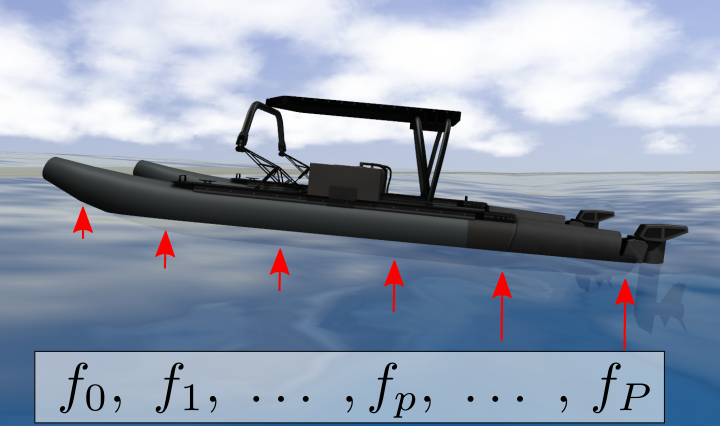
\includegraphics[width=\FigWidth\textwidth]{images/wamv_grid_v2.png}
  \caption{Illustration of wave-induced forces on USV. Force vectors represent restoring forces at discrete grid points along the WAMV demi-hull.}
  \label{f:wamv_grids}
\end{figure}

This approach to approximating the influence of ocean waves is a simplification intended to balance physical fidelity and visual realism with real-time execution requirements.  The result is consistent simulated motion and sensor feedback to exercise the pertinent aspects of autonomy, particularly motion control and sensor-based perception.  To preserve real-time execution, the model neglects wave influence factors typically included in applications where the precise motion of a particular vessel or structure design are of critical importance, e.g., studies that include slamming, green water on deck and dynamic stability.  A variety of naval architecture design software applications provide methods to assess the affect of vessel design on resulting motion, but these solutions typically run much slower than real-time.  Previous work by the authors  compared the proposed approach with a commercial naval architecture design software package under similar sea conditions, taking into account model forces and motions to quantify the trade-offs in complexity and fidelity \citep{malia18modeling}. The results quantified the fidelity differences between the approaches and demonstrated that the proposed method could sufficiently exercise robotic autonomy while executing in real-time.   

%common hydrodynamic problems in seakeeping and vessel design.  As an example, vessel response in irregular waves is often formulated using potential flow and decomposed into components of diffraction and radiation potentials that generate corresponding forces \citep{newman77hydrodynamics,faltinsen90sealoads}.  The radiation effects result from fluid motion in response to vessel motion, generating forces due to vessel motion in a quiescent fluid.  These forces are accounted for in the added mass and damping terms described in Section~\ref{s:hydro}.  The diffraction effects result from wave interaction with the vessel body, generating forces on a stationary vessel in an oscillating wave field.  The diffraction effects can be further decomposed into incident and scattering effects.  The Froude-Krylov hypothesis simplifies this formulation by asserting that the body is sufficiently small as to not affect the pressure field of the wave, which enables neglecting the scattering effects.  Under these conditions the incident potential term is referred to as the Froude-Krylov force and approximates the excitation force due to the pressure field of the incident wave.  
% Need a check on my edits above

%Modeling approaches such as the potential flow formulation above provide an approximation of vessel response with additional fidelity compared to the simplified method we describe in Algorithm~\ref{a:waves}.  Higher fidelity methods are warranted for applications where real-time execution is not a priority and the details of the motion of a particular vessel or structure design are of critical importance.  Such applications consider effects such as slamming, green water on deck and dynamic stability.  A variety of naval architecture design software applications provide capabilities to assess the affect of vessel design on resulting motion.  Previous work by the authors \citep{malia18modeling} compared the proposed approach with a commercial naval architecture design software package under similar sea conditions, taking into account model forces and motions to quantify the trade-offs in complexity and fidelity. The results showed that while there is a reduced fidelity for the Gazebo-based approach, it nonetheless demonstrates the ability to sufficiently exercise the robotic autonomy while executing in real-time.  

\subsection{Wind Forces}
The model used for simulating the wind environment---consisting of horizontal wind speed ($V_w$) and direction ($\beta_w$)---is described in Section~\ref{s:wind_model}.  We consider the influence of this wind on the maneuvering degrees-of-freedom of the model.  We neglect the wind-induced motion in heave, pitch and roll.  While the influence on heave and pitch are typically very small, for certain vessels, under certain conditions, the wind can have an effect on roll.  For such cases the same coefficient-based model presented below can be extended.

We adapt the model and notation described by \citet{fossen94guidance}.  The relative (apparent) wind velocities are
\begin{IEEEeqnarray}{rCl}\IEEEyesnumber\label{e:relwind}
u_{rw} & = u - u_w \IEEEyessubnumber \\
v_{rw} & = v - v_w \IEEEyessubnumber 
\end{IEEEeqnarray}
where $u_w$ and $v_w$ are the x and y components of the simulated wind velocity in the vessel body frame, expressed as
\begin{IEEEeqnarray}{rCl}\IEEEyesnumber\label{e:wvel}
u_w & = V_w \cos(\beta_w - \psi) \IEEEyessubnumber \\
v_w & = V_w \sin(\beta_w - \psi). \IEEEyessubnumber 
\end{IEEEeqnarray}
The surge, sway and yaw components of the wind force vector ($\bm{\tau}_{wind}$ in \eqref{e:fossenmodel}) are dependent upon the apparent wind and the coefficients for each mode.  For symmetrical vessels, these wind coefficients can be considered constant.  Using dimensional wind coefficients $\bar{c}_x$, $\bar{c}_y$ and $\bar{c}_n$ we express the forcing terms as
\begin{IEEEeqnarray}{rCl}\IEEEyesnumber\label{e:wind} 
  X_{wind} &=&\bar{c}_x u_{rw} |u_{rw}| \IEEEyessubnumber \\
  Y_{wind} &=& \bar{c}_y v_{rw} |v_{rw}|\IEEEyessubnumber \\
  N_{wind} &=& -2.0 \bar{c}_n u_{rw} v_{rw}. \IEEEyessubnumber
\end{IEEEeqnarray}

This wind forcing model is implemented as another standalone Gazebo plugin.  At runtime the user specifies the wind characteristics---mean direction and speed---and the vessel-specific wind coefficients in \eqref{e:wind}. The wind speed and direction at simulation time is calculated according to the wind generation model in \eqref{e:sim2}, the components of the apparent wind are calculated in the vessel body-frame and the resulting forces from \eqref{e:wind} are applied to the simulated vessel for inclusion in the next cycle of the physics engine update.

Analogous to the hydrodynamic model, this approach to representing wind-induced forces is generally applicable to surface vessels and a vessel-specific application requires estimation of the wind coefficients.  For the \wamv{} model, wind coefficients have been estimated based on experimental testing \citep{sarda16station}.  We use these numerical values for the \wamv{} for the purposes of the VRX challenge reference implementation.  

\subsection{Propulsion Forces}
The propulsion system consists of a set of vessel-mounted thrusters to implement vessel motion control by generating external forces on the vehicle.  Design of the propulsion system includes specification of the thruster type,  thruster characteristics, and thruster location on the vessel.  To accommodate user-defined configurations, we model the force from an individual thruster as a function of a thrust command between -1.0 (full reverse) and 1.0 (full forward).  At each time step the resulting external force is included in the model according to \eqref{e:fossenmodel}.  Implemented as a Gazebo plugin, this force is applied at the geometric location of the propeller joint as illustrated in \figref{f:thrust}.  Each thruster can also be articulated by commanding the angle of the thruster relative to the mount, allowing for the possibility of vectored thrust solutions.  The motion of the angular articulation is simulated through a proportional-derivative controller to move the thrust vector to the desired location with temporal dynamics representative of typical electromechanical dynamics.

\begin{figure}[hbt!]
  \centering
  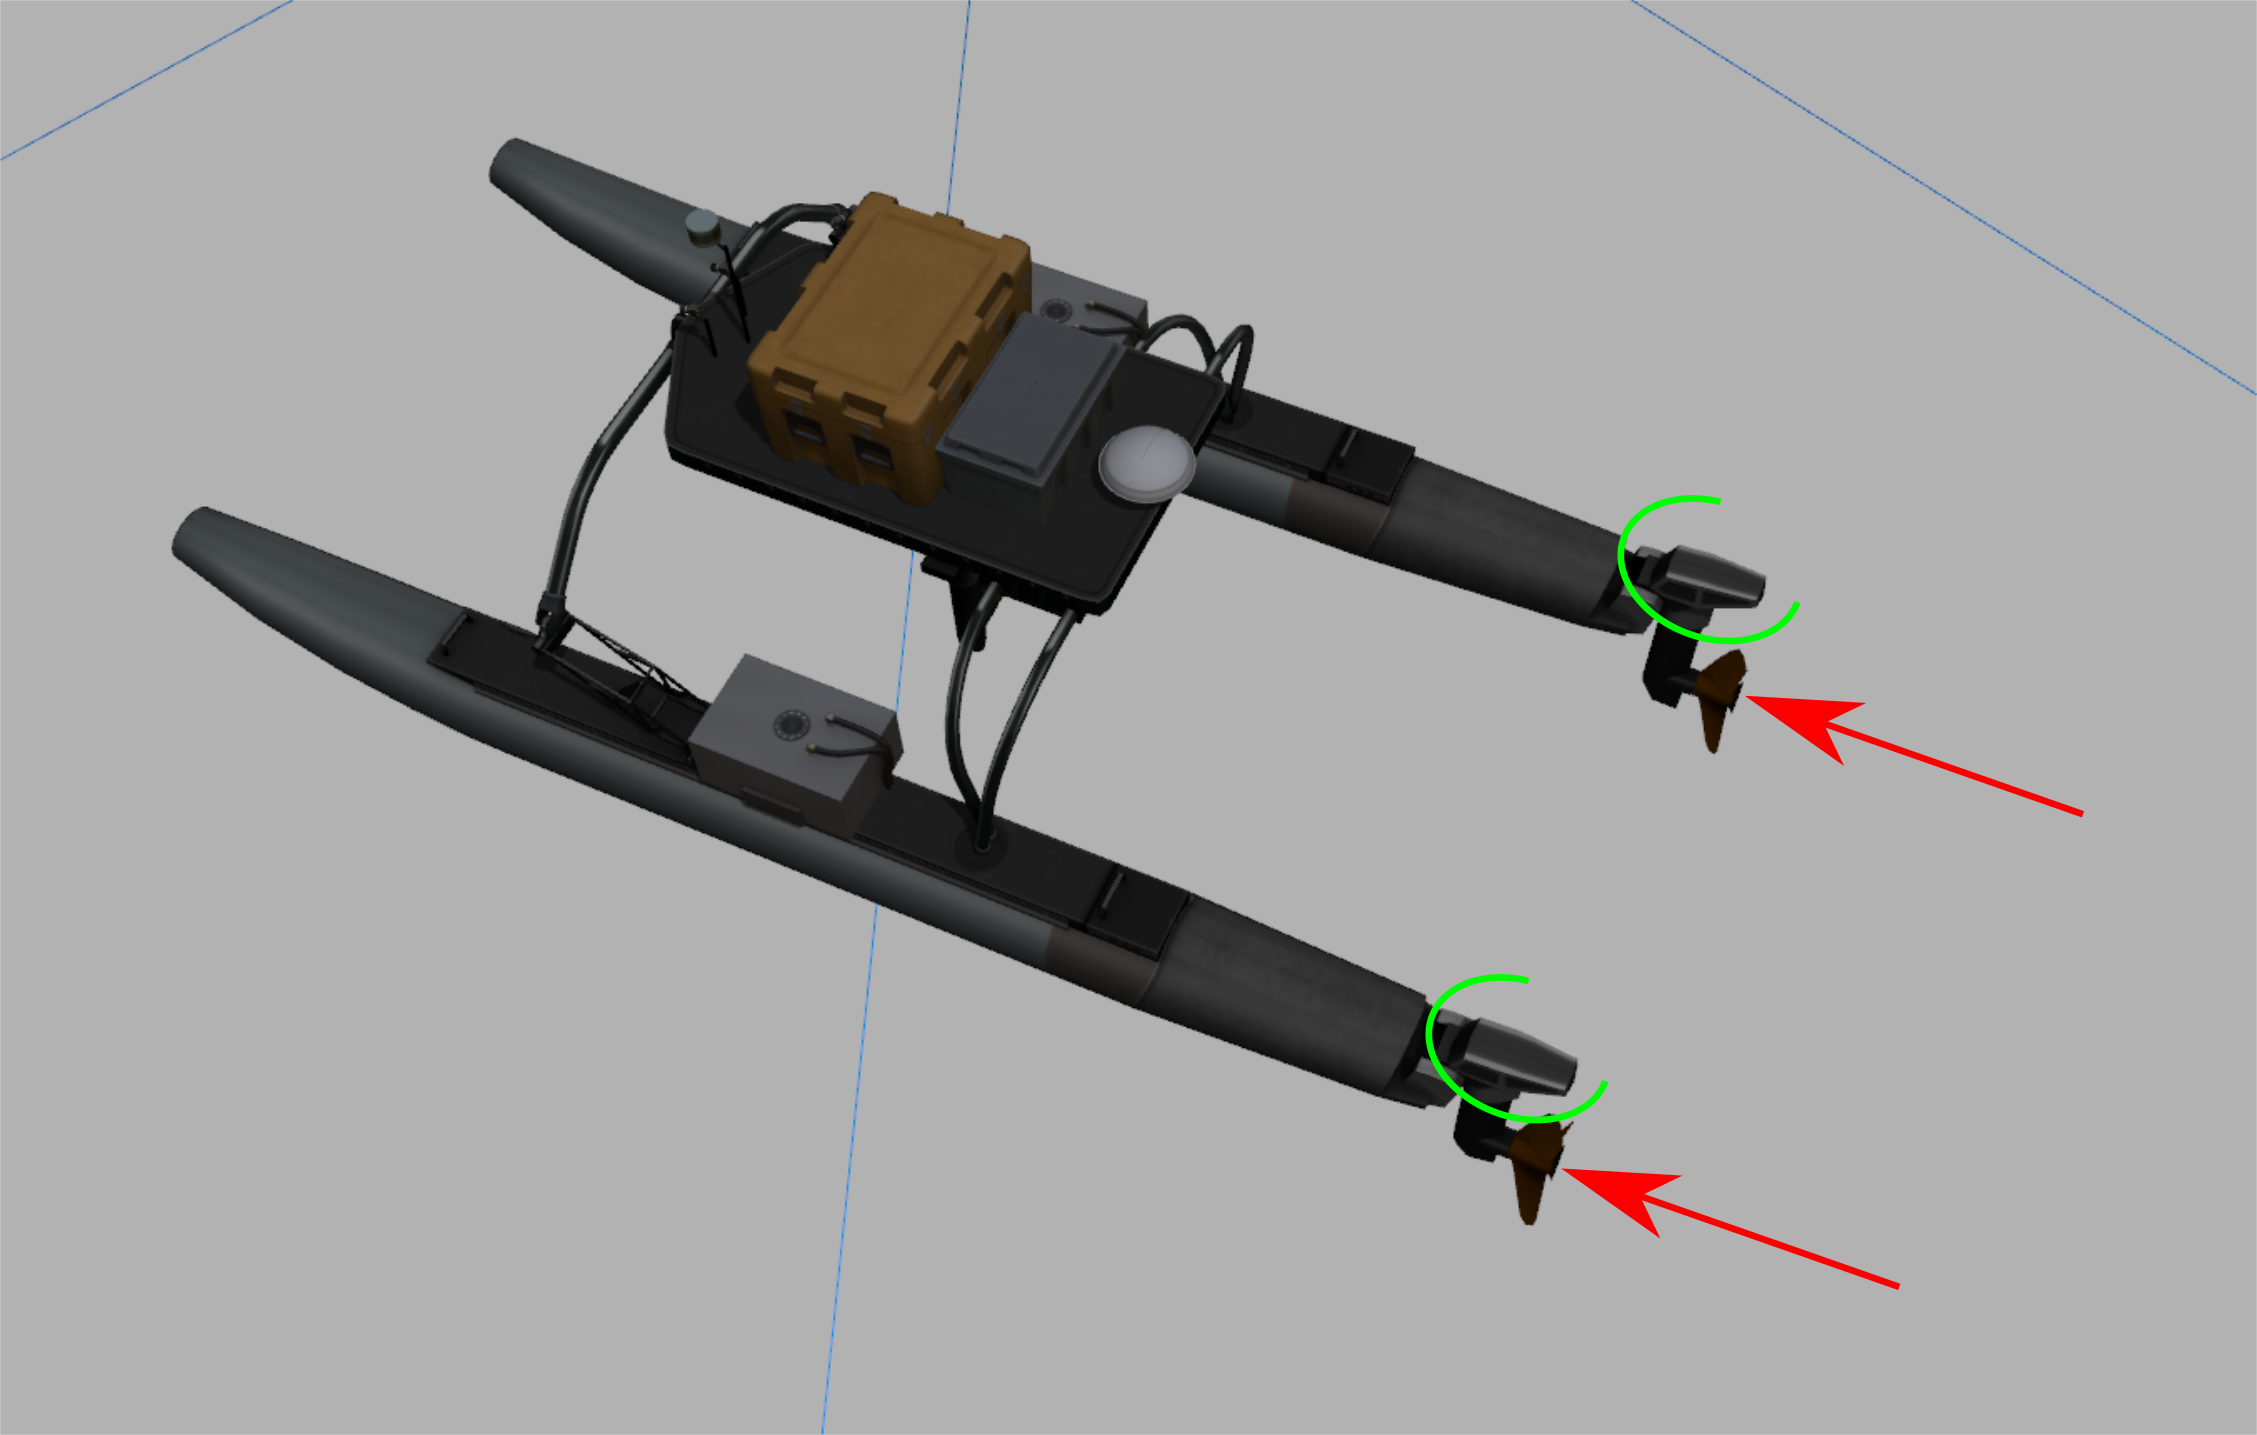
\includegraphics[width=\FigWidth\textwidth]{images/thruster_annote.png}
  \caption{Illustration of propulsion forces for a two-thruster configuration.  Two independent forces are applied to the virtual body as indicated by the red arrows.  The angle of the each thruster relative the mounting point can also be controlled to allow for vectored thrust, as indicated by the green arcs.}
  % Moved to comment: "This image needs work."
  \label{f:thrust}
\end{figure}

While \figref{f:thrust} shows a typical configuration with two thrusters at the stern of the vessel, users may add multiple thrusters at other locations to reflect other possible propulsion system designs.  For example, an additional bow or lateral thruster is often added for additional control authority; alternately, a four-thruster configuration with angled thrusters at the bow and stern of each hull can be implemented when maneuverability is prioritized over speed and efficiency.  

The characteristics of an individual thruster are specified by a user-defined relationship between commanded effort and the resulting thrust force.  Two static mappings are included; custom mappings are supported for more specific cases.  The first mapping is a linear mapping where the command values (-1.0 to 1.0) are scaled linearly to the user supplied parameters for maximum forward and reverse thrust values.  

The second, non-linear static mapping uses generalized logistic functions (GLFs) to approximate the relationship between command and force often provided as the result of static bollard-pull tests.  The GLF is parameterized as 
\begin{equation}
  T = A + \frac{K-A}{\left(C+\exp(-B(x-M))\right)^{1/\nu}}
  \label{e:glf}
\end{equation}
where $T$ is the thrust in Newtons; $x$ is the commanded effort; and $A$, $K$, $C$, $B$, $M$, and $\nu$ are user-defined constants used to specify the GLF. To capture the asymmetry associated with forward and reverse, two independent GLFs are used, one for positive commands (0 to 1.0) and a second for negative commands (-1 to 0).  The user-specified functional parameters allow the thrust model used to approximate a wide variety of thruster designs based on empirical data.

To illustrate this process we specify the GLF thrust mapping to approximate the  steady-state bollard-pull experiments reported by \citet{sarda16station}.  To identify the GLF parameters, a Nelder-Mean simplex optimization was performed to minimize the squared error between the model and the GLF expressions \eqref{e:glf} as a function of the GLF parameters.  The results are shown in \figref{f:fit}.
\begin{figure}[h]
  \centering
  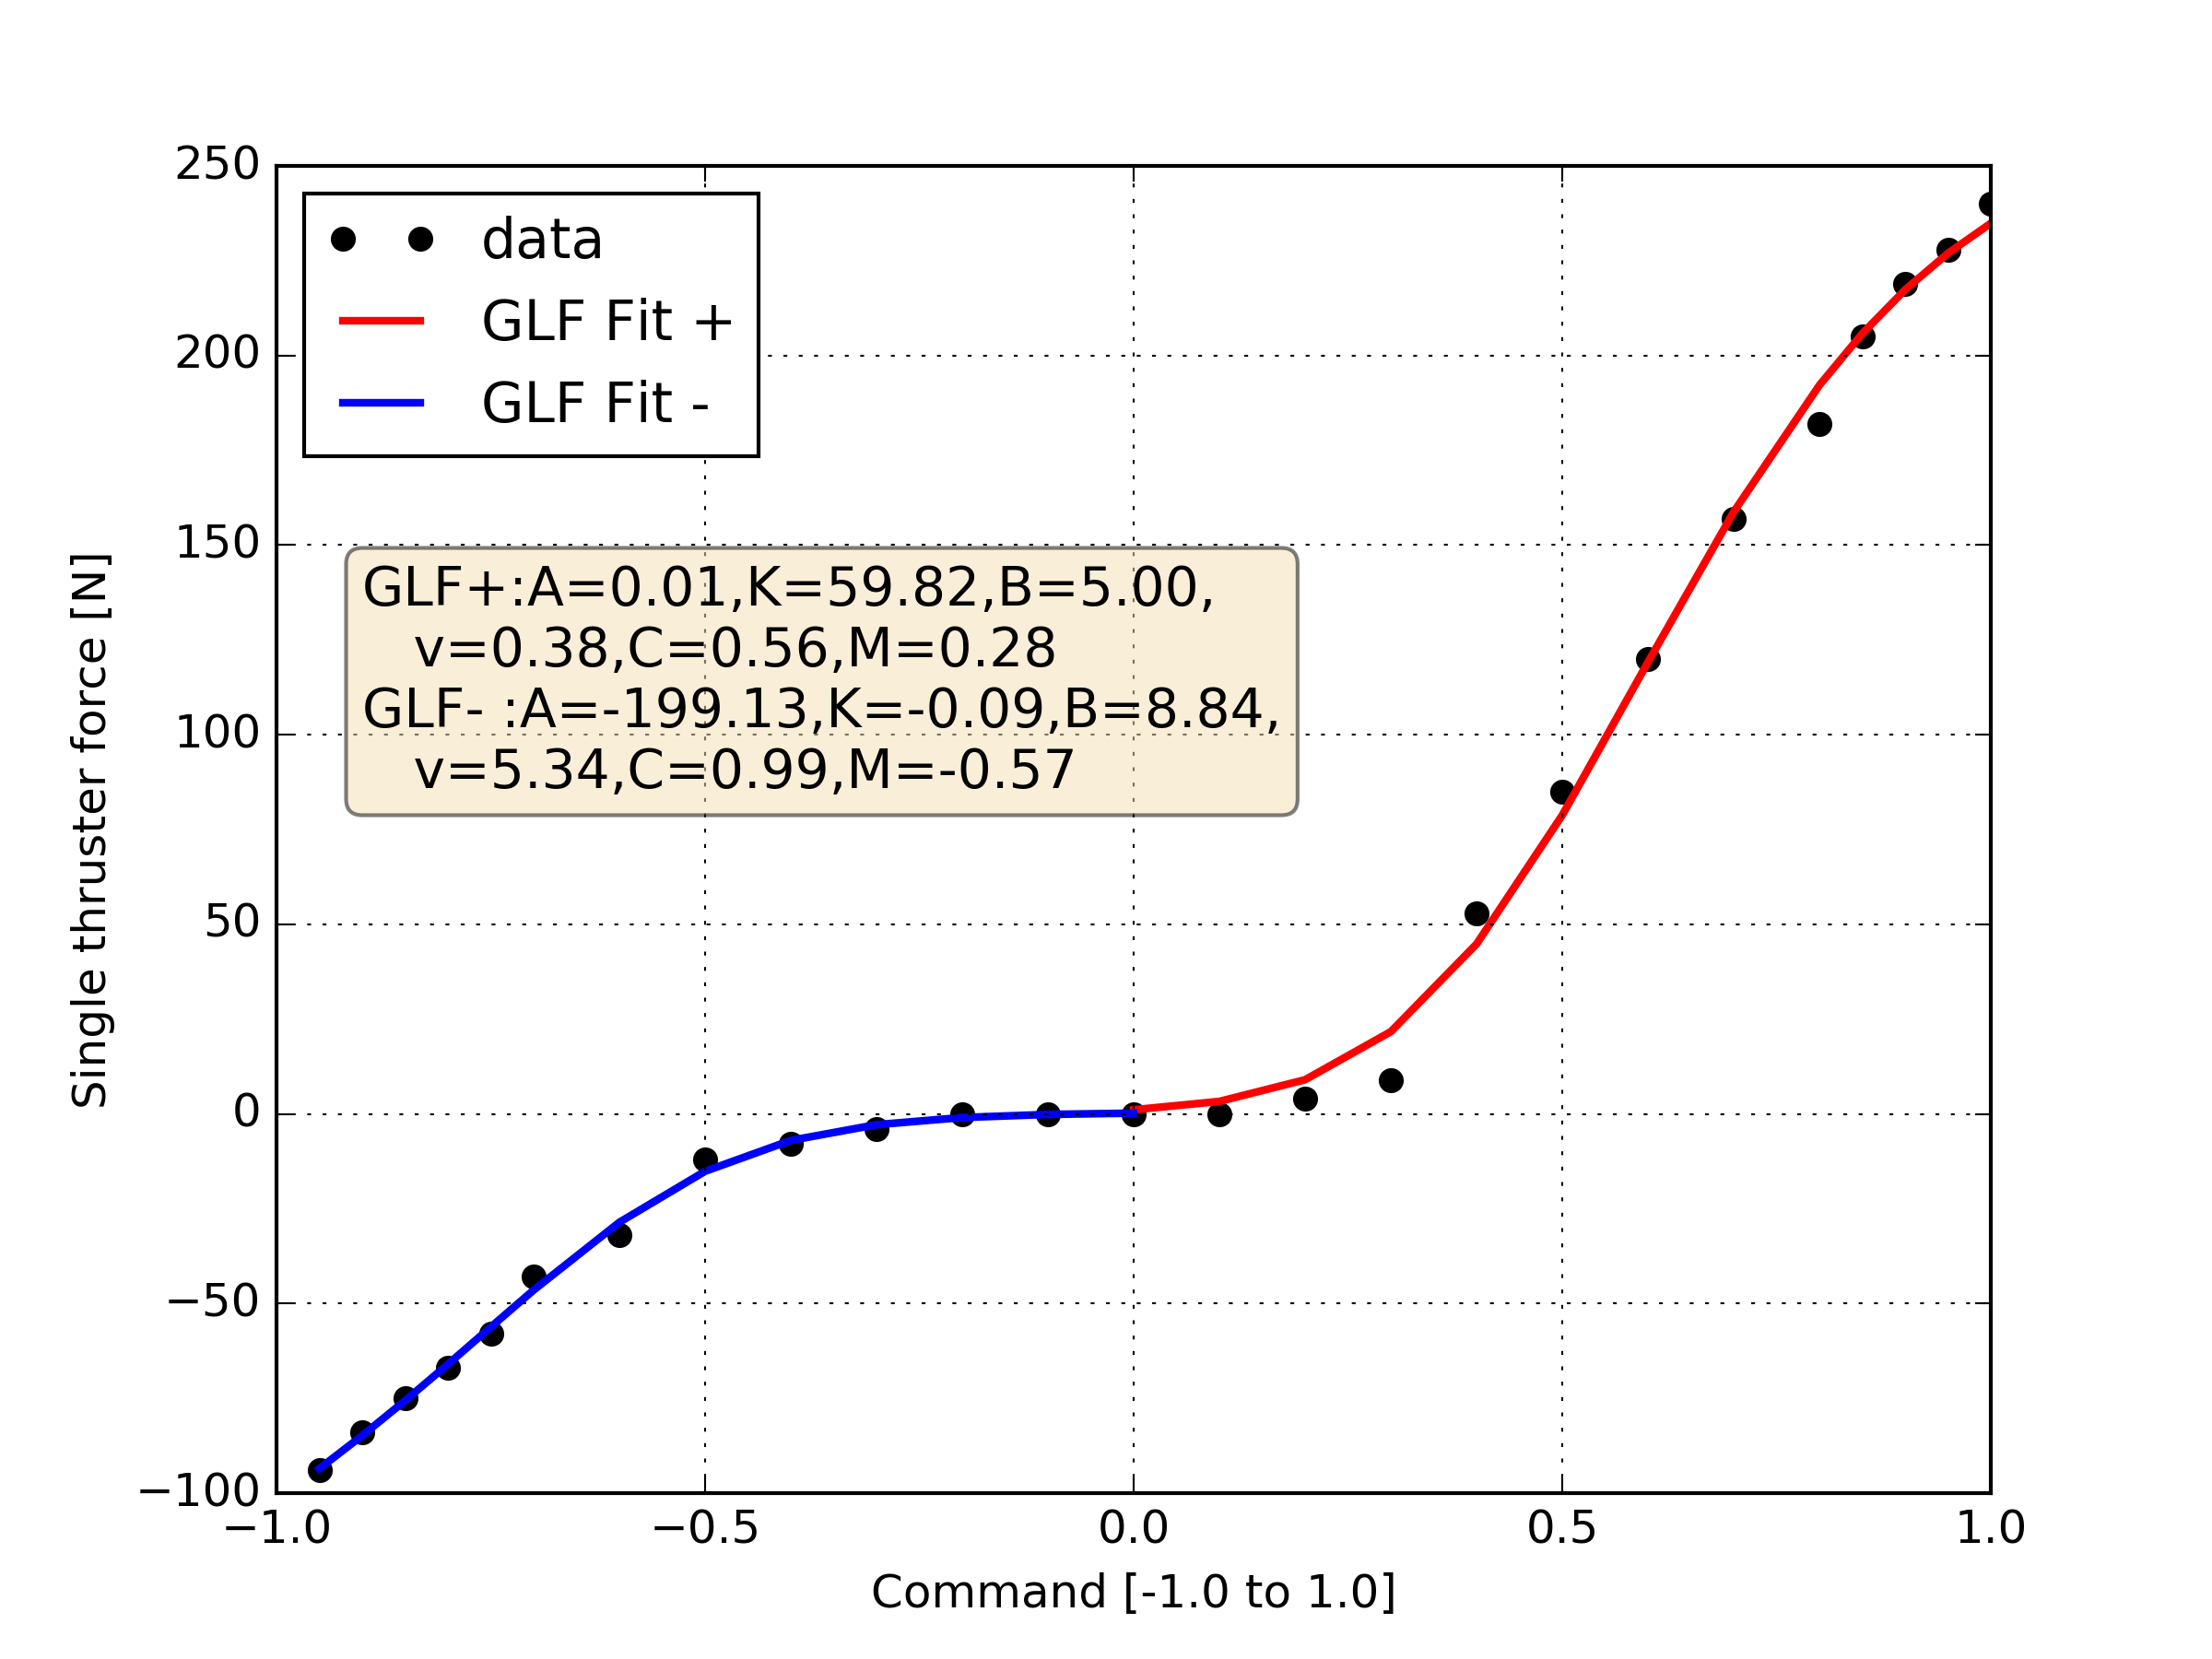
\includegraphics[width=\SFc\textwidth]{images/wamv_glf_annote2.png}
  \caption{Generalized logistic function fit of empirical  bollard-pull thrust performance data from \citep{sarda16station}.}
  \label{f:fit}
\end{figure}

This approach to simulating propulsion force approximates the steady-state non-linearities to exercise the motion controllers under test.  However, it does not address effects such as transient thruster dynamics for slow-speed control described by \citet{whitcomb99development}, varying advance ratios due to forward vessel speed for high-speed operation or changes in thrust during turning due to the changing inflow angle, which can generate meaningful side force.  Such additions to the propulsion model can be readily implemented, but rely upon the availability of more detailed propulsion characterization.
%
\color{red}
\section{Model and Simulation Verification}
%
To confirm that our vehicle model captures the correct \emph{behavior} of the \wamv{}, we have simulated a number of standard maneuvering and seakeeping tests in the VRX environment. The purpose of these tests is not to validate our model against the actual \wamv{} but rather to confirm that our model captures realistic behavior and the correct dependencies on the wave and propulsion inputs. This means that for incident waves, we expect a measurable but bounded motion response that increases as the wave height increases. For the propulsion input we expect a thrust difference between the two propellers to cause the vehicle to turn with the turning radius decreasing as thrust differential increases.

The first set of simulations were a series of seakeeping tests. The \wamv{} response was simulated using our vehicle and incident wave field models. In the simulation the \wamv{} had no controller setpoints and almost no thrust. The incident wave field was monochromatic, longcrested waves, that had a period of \unit[6]{s} and wave heights that varied from \unit[0]{m} up to \unit[2]{m} across the set of simulation runs. Assuming the deep water dispersion relationship, these waves had a wavelength of approximately \unit[56]{m} and thus a wavelength-to-vehicle length of roughly $14$. The largest wave has a wave steepness, wave height to wave length ratio, of $1/30$ which is typical for seakeeping tests. These conditions were chosen because they represent a wave environment ranging from a Sea State $1$ to $4$. (reference one of your sea state table papers???)

Figure~\ref{f:head_seas} shows the amplitude of the oscillatory heave, pitch, and roll responses of the \wamv{} to head seas under these wave and operating conditions.
%
\begin{figure}[h]
  \centering
  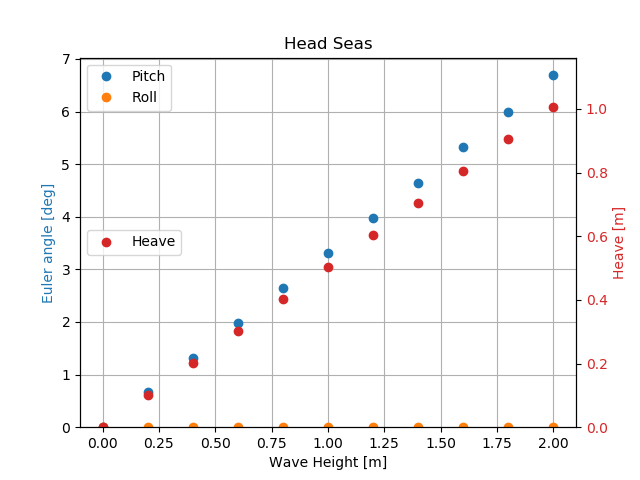
\includegraphics[width=\SFc\textwidth]{images/2020_08_25_head_seas_001.png}
  \caption{Simulation results for wave induced motion in head seas.}
  \label{f:head_seas}
\end{figure}
%
Each simulation was run for \unit[60]{s} resulting in roughly $10$ wave encounters. The amplitude of the oscillatory motion response in each degree-of-freedom was determined using only the last XX wave encounters to avoid being influenced by the initial transients. The roll and pitch amplitude is plotted using the left y-axis scale in the figure and the heave amplitude is plotted against the right y-axis scale. Since these cases correspond to head seas, we expect to see an increasing amplitude in pitch and heave and very little response in roll. The figure shows that the pitch and heave amplitude responses of the \wamv{} increased as the wave height increased. Furthermore, the responses show that the \wamv{} is contouring to the passing waves as typically happens when the wavelength is considerably longer than the vehicle length. This means that the pitch angle matches the local slope of the wave and the heave displacement matches the wave amplitude. For the largest wave simulated, the maximum wave slope, given by $ka$, is \unit[6.4]{$^\circ$} and matches the simulated amplitude of the oscillating pitch. The heave amplitude response of the \wamv{} for this wave equals \unit[1]{m} which is the wave amplitude. Finally, the roll amplitude remains very small as the wave height increases. There is a small response since the vehicle does not remain perfectly aligned in a head seas condition, instead yawing slightly since there is no heading controller during these simulations.

Figure~\ref{f:beam_seas} shows the heave, pitch, and roll response amplitudes of the \wamv{} again but this time for beam seas. The formatting of the figure axes and data is the same as Fig.~\ref{f:head_seas}.%
%
\begin{figure}[h]
  \centering
  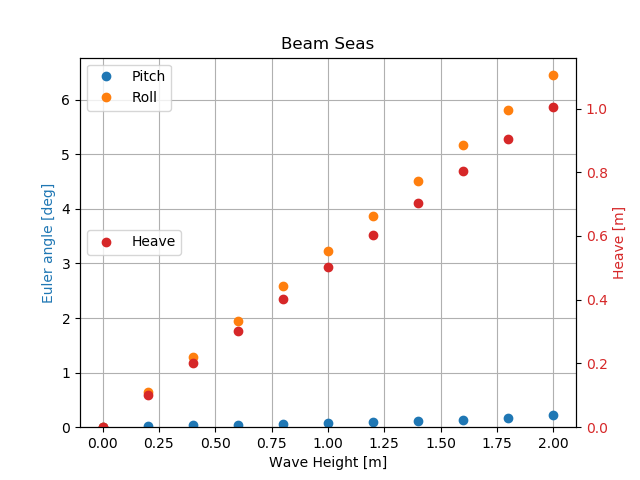
\includegraphics[width=\SFc\textwidth]{images/2020_08_25_beam_seas_001.png}
  \caption{Simulation results for wave induced motion in beam seas.}
  \label{f:beam_seas}
\end{figure}
%
Since this is a beam seas wave environment, we expect to see a vehicle response in roll now instead of pitch while still seeing a heave response. The figure shows that the simulated roll and heave amplitudes of the oscillatory response of the \wamv{} increase as the wave height increases and that the vehicle motion is again contouring to the passing wave. The ratio of the pitch amplitude to the wave slop is again unity as is the ratio of the heave amplitude to wave amplitude. Finally, consistent with a beam sea, the pitch response of the \wamv{} is much smaller than the roll response.

The second set of simulations were a series of maneuvering tests involving turning circles. Our vehicle model was used to simulate the \wamv{} response to a thrust differential in calm water. By having the thrust command of the port and starboard propellers be different, a yawing moment is experienced by the vehicle and it should follow a circular trajectory. In each simulation, the magnitude of the overall thrust command was set to 0.75\% of the maximum. This made the surge velocity roughly constant across the simulations. Each simulation was run for \unit[60]{s}, so the distance travelled by the vehicle is approximately equal for each run shown.

Figure~\ref{f:manuevering} shows the \wamv{} trajectory for each of the simulations. The legend shows what the thrust command was for the port and starboard propeller for each run, with each run denoted by a different color. The trajectories clearly show the correct behavior that a thrust differential causes the \wamv{} to perform a turn. Furthermore, the model also captures the correct behavior that as the thrust differential increases, the \wamv{} undergoes a tighter turn and has a larger yaw rate.
\begin{figure}[h]
  \centering
  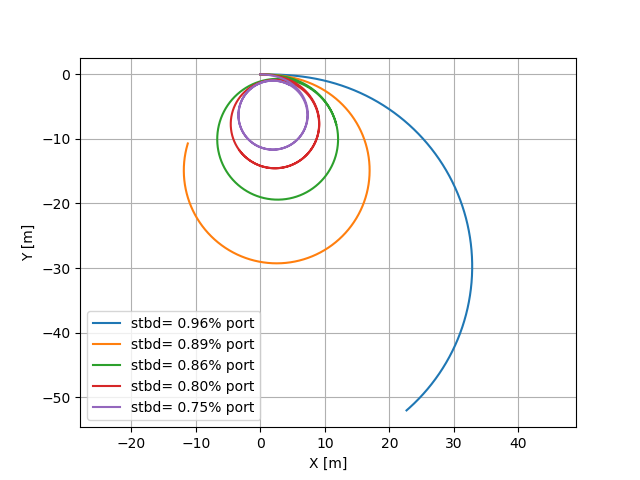
\includegraphics[width=\SFc\textwidth]{images/2020_08_25_manuevering_000.png}
  \caption{Simulation results for maneuvering in calm water.}
  \label{f:manuevering}
\end{figure}

The results of our simulation runs confirm that our unified model displays the correct type of behavior in the seakeeping heave, roll, pitch degrees-of-freedom and the maneuvering surge, sway, yaw degrees-of-freedom. Our model captures the correct behavior that incident waves cause the \wamv{} to undergo oscillatory motion, that the amplitude of these motions increase with increasing wave height, and that the vehicle contours to the wave. Our model also captures the correct behavior of a turning circle maneuver caused by a thrust differential where the diameter of the turning circle decreases as the thrust differential increases.\color{black}
%
\section{VRX Reference Implementation}
%
Launched in 2012 with support from the Office of Naval Research, the Maritime RobotX Challenge is hosted biannually by RoboNation to promote research and advancement in autonomous surface vehicles, as well as to encourage student interest and foster relationships within the robotics community. Participating teams compete to design and implement systems capable of accomplishing a variety of tasks ranging from basic navigation and control to more complex operations involving obstacle avoidance, perception and underwater object retrieval.

%Since its inception, RobotX has drawn interest from well over a dozen university robotics teams at each of its event. The latest of these, held in 2018 at Sand Island Boat Launch in Honolulu, involved contributions from 15 universities from around the Pacific Rim. 
%
The purpose of the VRX challenge is to provide competitors with the opportunity to prototype and test software solutions in advance of physical on-water deployments. A major goal of the project is to facilitate improved performance in the physical competition. As such, it implements a suite of models and plugins that closely mirrors the location, course elements, and types of tasks encountered by participants in RobotX 2018. \figref{f:robotx_vrx} shows a visual comparison of an example vehicle and elements from RobotX alongside a similar scene rendered in the VRX environment with Gazebo. %To encourage engagement with the platform as well as to underscore its utility with respect to preparing for RobotX, we employ these components in the creation of the VRX Competition-\footnote{\url{https://robotx.org/index.php/about/about-virtual-robotx}}---a virtual competition that parallels the structure and approach of the RobotX Challenge. 

\begin{figure}[hbt!]
  \centering
  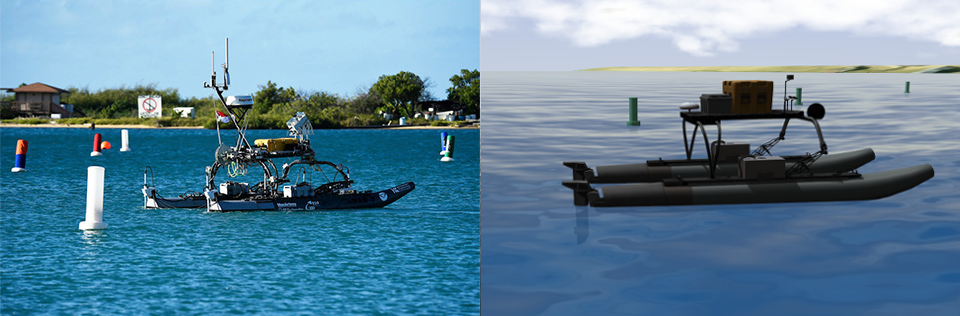
\includegraphics[width=\FigWidth\textwidth]{images/robotx_vrx_wamv.png}
  \caption{A visual comparison of a physical \wamv{} and course elements from RobotX 2018 (left) with a similar scene rendered in the VRX environment using Gazebo (right).}
  \label{f:robotx_vrx}
\end{figure}

The first VRX Competition was held in November 2019. Similar to RobotX, the VRX Challenge is organized around a series of tasks that evaluate autonomous navigation and perception capabilities of participants' solutions.  These tasks include station-keeping, waypoint guidance, object localization and characterization, navigation and rules of the road, and docking.  The VRX environment also serves as a proof of concept for the theory of operations herein described. Tasks require teams to develop solutions that correctly compensate for the influence of waves and wind when controlling the motion of the vehicle. The station-keeping and path planning tasks, in particular, bring this requirement into relief.  In order for these tasks to provide useful evaluations of participant solutions, the VRX environment must succeed in simulating the impact of wind and wave forces with sufficient fidelity and speed.  The object localization and characterization task isolates environmental effects on perception, and therefore relies heavily on the availability of synchronized visual and physical models. Finally, the more complex navigation and docking tasks test the ability of the VRX environment to render a real-time simulation that gives a sufficiently faithful approximation of environmental influence on both motion control and perception effects at the same time\footnote{A complete description of the VRX 2019 challenge tasks is available at \url{https://bitbucket.org/osrf/vrx/wiki/documentation}}.    

\figref{f:sandisland_wind} and \figref{f:dock_waves} demonstrate the combined effect of our environment and vehicle models within the VRX simulation environment. \figref{f:sandisland_wind} depicts the base Sand Island world on which the competition is built, including course elements and the \wamv{}. The inset graph included in the display shows the wind speed varying over time in accordance with user specified parameters and the model given in Section~\ref{s:wind_model}. \figref{f:dock_waves} was created from the Dock task plugin using a peak period of $5$ seconds and a gain ratio of $0.7$. The scene illustrates the effect of the wave field on vehicle motion as well as the disturbances to the perception system produced by the resulting pitch, roll and heave of the vehicle.  

\begin{figure}[hbt!]
  \centering
  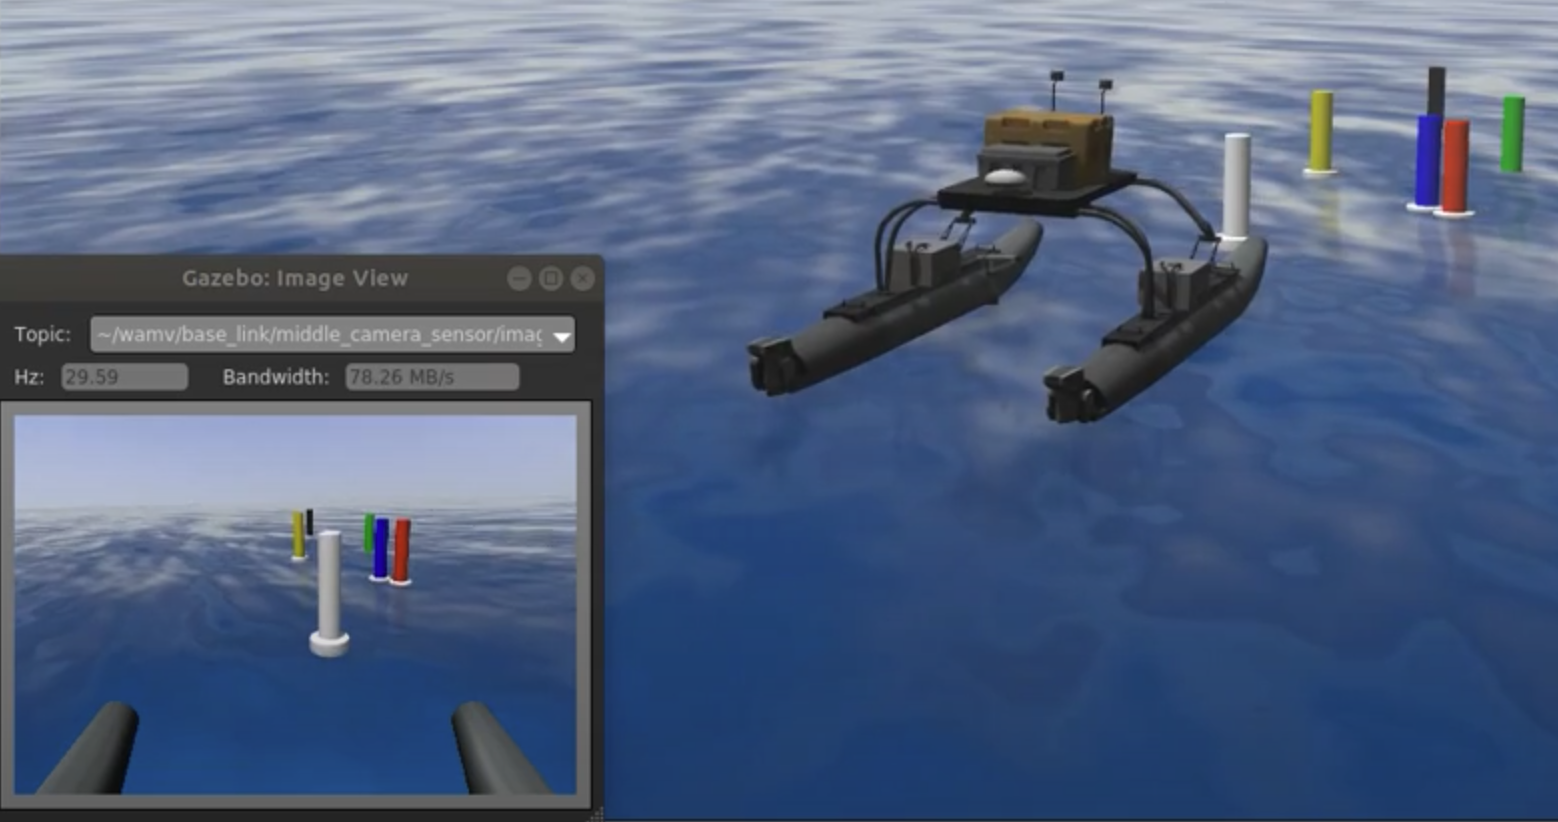
\includegraphics[width=\FigWidth\textwidth]{images/perception_task.png}
  \caption{The VRX Competition Perception task tests the ability to identify the number and type of markers that appear in the vehicle's point of view during a short time interval. The vehicle remains fixed along the $x$ and $y$ axes but is still subject to environmental forces that may cause it to pitch, roll and heave during the task.}
  \label{f:perception_waves}
\end{figure}

\begin{figure}[hbt!]
  \centering
  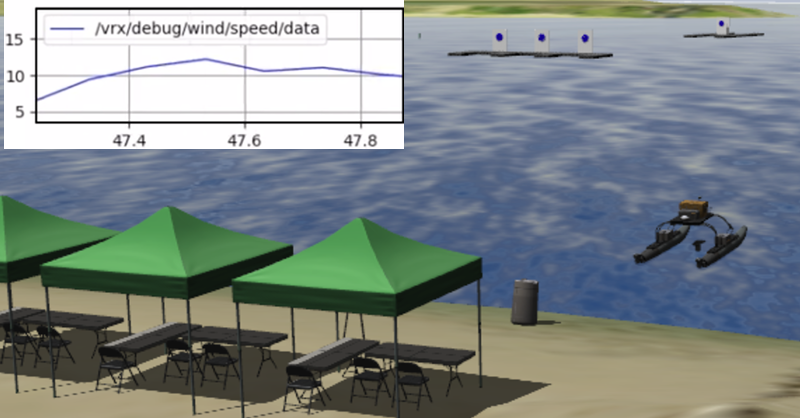
\includegraphics[width=\FigWidth\textwidth]{images/sand_island_beach_wind.png}
  \caption{The VRX Sand Island world rendered in Gazebo with a plot of wind speed over time.}
  \label{f:sandisland_wind}
\end{figure}

\begin{figure}[hbt!]
  \centering
  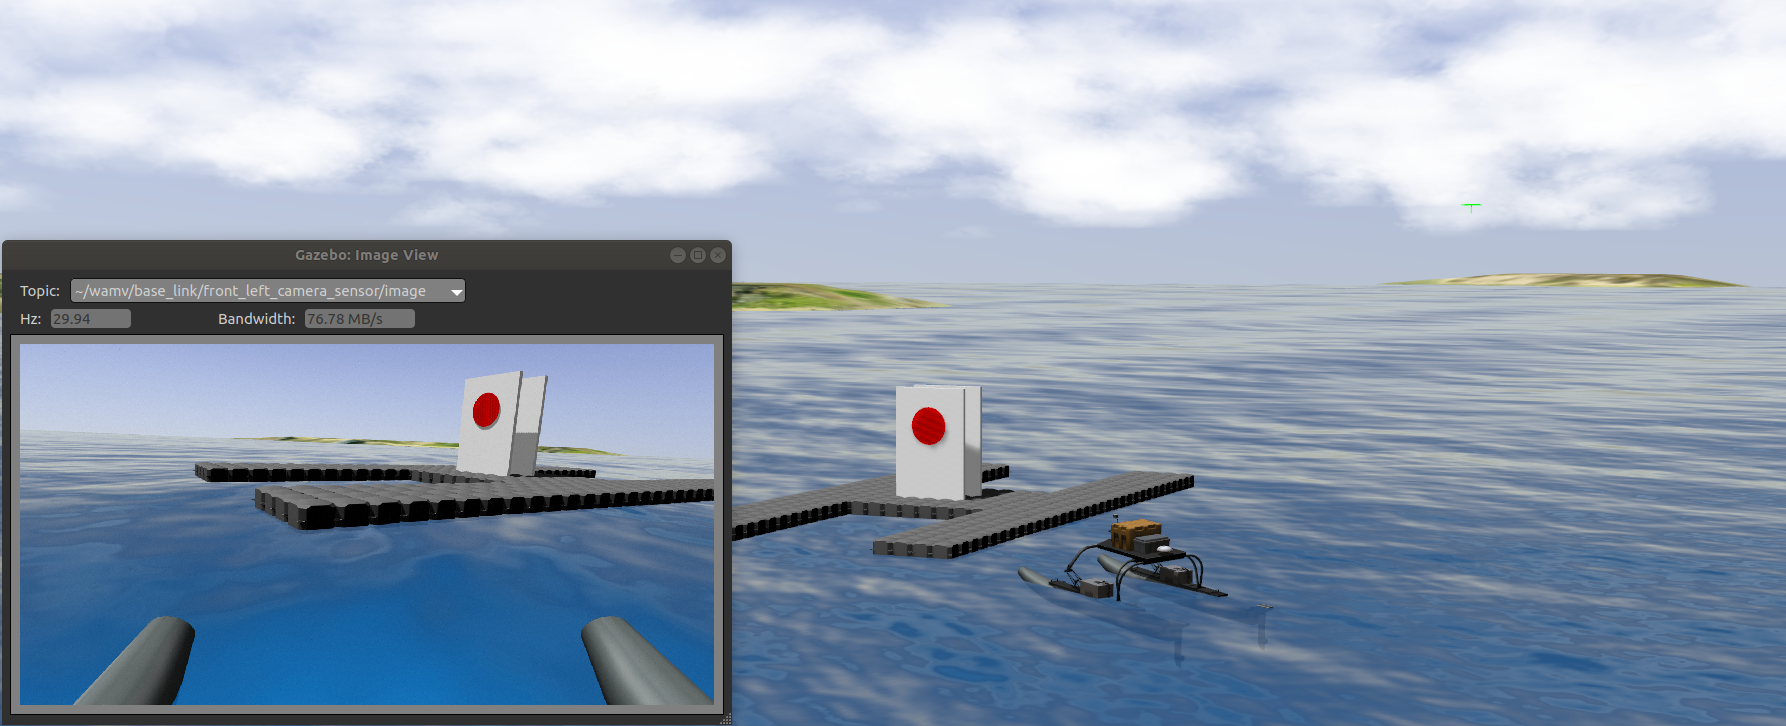
\includegraphics[width=\FigWidth\textwidth]{images/waves_sync.png}
  \caption{The VRX Competition Dock task with a non-trivial wave environment ($K = 0.7$, $T_p = 5$). Note the \wamv{} is slightly rolled and pitched due to wave forcing, and the effect of this disturbance is reflected in the camera view.}
  \label{f:dock_waves}
\end{figure}

\begin{figure}[hbt!]
  \centering
  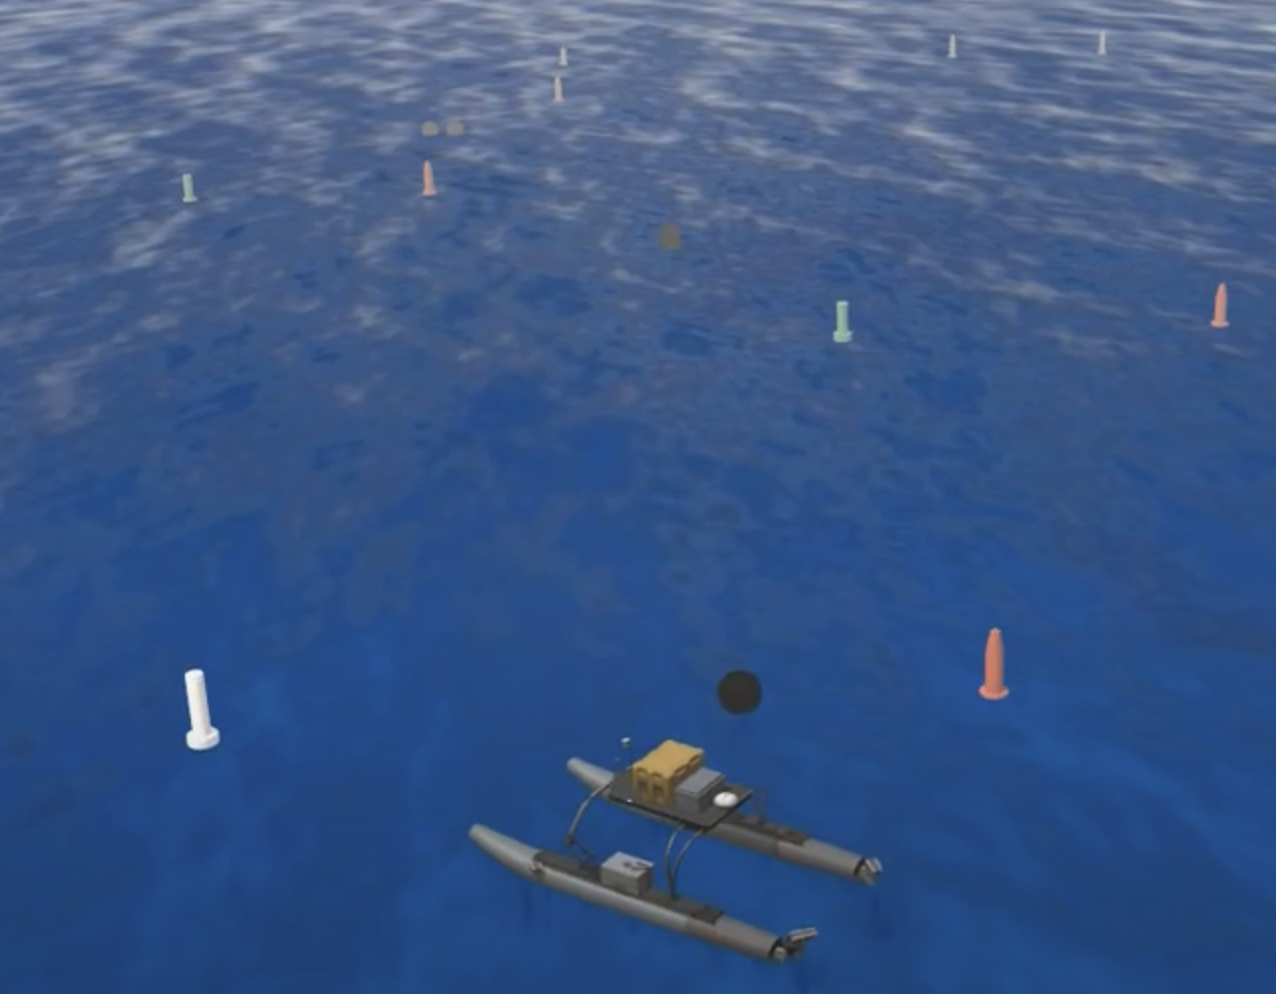
\includegraphics[width=\FigWidth\textwidth]{images/navigation_wide_fog_2.png}
  \caption{The impact of fog on VRX Competition Navigation task. As the vehicle enters the course, the color of distant markers is obscured by fog and appears faded. Similarly, black spherical obstacles are clearly visible up close, but rendered gray in the distance, making them difficult to distinguish from the water surface. }
  \label{f:navigation_fog}
\end{figure}

\section{Conclusion}

In this article we describe the theory of operation of a free and open source robotic simulation environment designed specifically to support rapid development, testing and evaluation of new autonomy solutions for marine applications.  The contributions of this research are a wave model for visual and physical effects based on Gerstner waves and the two-parameter Pierson Moskowitz spectrum, a wind model to represent mean and variable (gust) components based on the generic spectral representation, a parameterized propulsion model, a six degree-of-freedom vessel model to capture environmental and control influence on vessel motion and sensor perception, and a demonstrative reference implementation: the new 2019 VRX challenge robot competition.

The VRX simulation is implemented as a set of Gazebo plugins, object models (visual, collision and rigid body representations), and environmental scenarios (world scenes) released as an open source project.  The simulation is highly parameterized, allowing users to specify the details of the environmental (wave and wind spectra constants), the vessel (hydrodynamic and wind coefficients), the propulsion (thruster location and authority) and the sensors (type and location). This parameterization generalizes the simulation so that it is adaptable to a variety of surface marine autonomy applications.

%As a specific proof-of-concept we present the configuration of these general purpose tools to create a virtual version of RobotX scenarios---the VRX challenge.

\section*{Acknowledgments}
This project was supported in part by the Department of the Navy, Office of Naval Research.  The VRX simulator is an open source project that welcomes community contributions.  We thank all the contributors for their time and energy.  A current list of contributors is maintained at \url{https://bitbucket.org/osrf/vrx/wiki/Contributors}.

This article extends prior work by the authors in the same subject \citep{bingham19toward} by improving the environmental disturbance models (wind and waves) to increase physical fidelity, refining the surface vessel manuevering and seakeeping model, \color{red} performing a number of seakeeping and maneuvering vehicle response verification tests, \color{black} and reporting the outcome of the first virtual robotics competition.

\bibliographystyle{frontiersinSCNS_ENG_HUMS} 

\ifoverleaf
\bibliography{bbing_master}
\else
\bibliography{../latexlib/bib/bbing_master}
\fi

\end{document}


